\documentclass{book}
\usepackage{graphicx} % Required for inserting images

\usepackage{amsfonts}
\usepackage{amsmath}
\usepackage{array}
\usepackage{graphicx}
\usepackage{subfig}
\graphicspath{ {./images/} }
\usepackage{pifont}
\usepackage{hyperref}
\usepackage{stackengine}
\newcommand\xrowht[2][0]{\addstackgap[.5\dimexpr#2\relax]{\vphantom{#1}}}
\usepackage{tikz}
\usetikzlibrary{matrix}
\usepackage{geometry}
\newgeometry{
left=   1 in,
bottom= 1.5 in,
right=  1 in,
top=    1 in
}


\title{V\&C Systems Notes}
\author{Riccardo Cappi}
\date{January 2024}

\begin{document}

\maketitle

\section{Disclaimer}
These are just my notes that I used to prepare for the exam. So, probably, there will be both spelling and conceptual errors. Feel free to contact me at riccardo.cappi@studenti.unipd.it if you find any errors. This is the github repo where you can find the latex files of the notes: \url{https://github.com/riccardocappi/Computer-Science-notes}\\\\
Unfortunately the notes for this course are \textbf{incomplete} :(

\tableofcontents

\chapter{Machine Learning Basics}
\section{What is Machine Learning}
\textit{A computer program is said to learn from experience E with respect to some class of tasks T and performance measure P, if its performance at tasks in T, as measured by P, improves with experience E.} Basically, Machine Learning is the field of study that gives computers the ability to learn without being explicitly programmed. In fact, we use Machine Learning when its impossible to \textbf{exactly formalise} the problem (and so to give an algorithmic solution) or when formulating a solution it's very complex and cannot be done manually.
\subsection{Main Learning Paradigms}
\begin{itemize}
    \item \textbf{Supervised Learning:}
    \begin{itemize}
        \item \textbf{Goal: }give the \textit{right answer} for each example in the data.
        \item Given a training set $\{(x^{(i)}, y^{(i)})\}$ we look for a function $h(\cdot)$ which is able to map in a predictive way $x^{(i)}$'s to $y^{(i)}$'s. It's called supervised learning because there is an expert that provides a \textit{supervision} assigning a label $y^{(i)}$ to each input $x^{(i)}$ 
        \item \textbf{Output: }Classification, regression.
        \item Use cases: Object recognition, Predicting pandemic, ... 
    \end{itemize}
    \begin{center}
        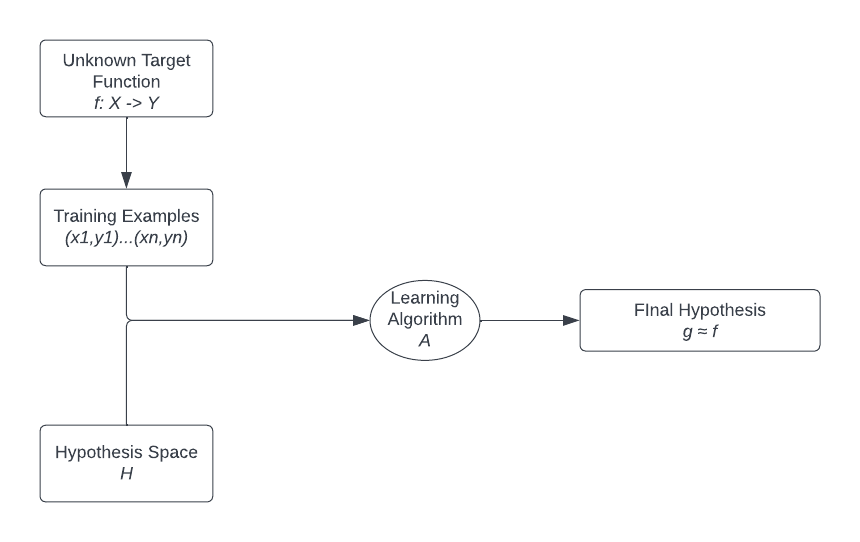
\includegraphics[scale=0.8]{images/Supervised Learning Diagram.png}
    \end{center}
    The \textit{Training examples} are generated according to the \textit{Target function $f$} (unknown). Once we have this set of pairs, we choose the \textit{hypothesis space}. The \textit{learning algorithm} (e.g a Neural Network) searches in the hypothesis space for a function $g$ that approximates the target function $f$.
    \item \textbf{Unsupervised Learning:}
    \begin{itemize}
        \item \textbf{Goal:} Find regularities / patterns on the data
        \item Given examples $\{x^{(i)}\}$, discover regularities on the whole input domain.
        \item There is no supervision.
        \item Use cases: Community detection in social media, user profiling, market analysis ...
    \end{itemize}    
    \item \textbf{Reinforcement Learning:}
    An \textbf{Agent} operates in an environment $e$, which in response to action $a$ (given by the agent) in the state $s$ returns the next state and a reward $r$ (which can be positive, negative or neutral).
    The goal of the Agent is to maximize a reward function.
    \begin{itemize}
        \item Use cases: Robotics, Games, ...
    \end{itemize}
    \begin{center}
        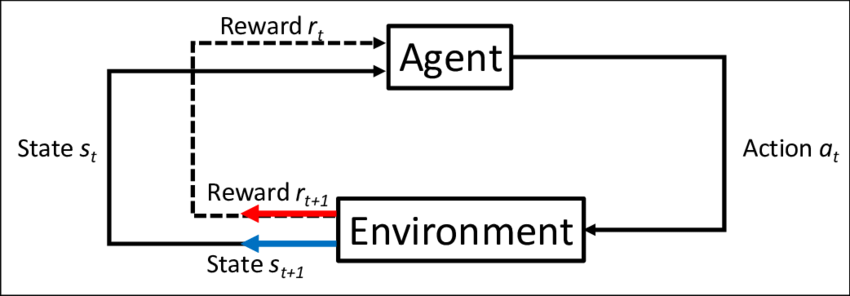
\includegraphics{images/Reinforcement learning.png}
    \end{center}
    \item \textbf{Other Learning Strategies:}
    \begin{itemize}
        \item Active Learning
        \item Online Learning, Incremental \& Continual Learning
        \item Weak Supervised Learning
        \item Self-supervised Learning
        \item Deep Learning and Representation Learning
        \item Federated Learning
    \end{itemize}
\end{itemize}

\subsection{Supervised Learning Keywords}

\begin{itemize}
\item \textbf{Input/Instance space x $\in X$:}
Representation of model's input (e.g. you can choose a Vector as a representation for your input). It contains all the possible inputs for a model. Suppose the model takes in a vector, $input = [x1, x2], x1,x2 \in [1,10]$, then we have $10^2$ possible inputs.
\item \textbf{Output space $y \in Y$:}
In supervised learning we want to perform a prediction based on the input. This prediction can be in the form of:
\begin{itemize}
    \item Binary Classification $y \equiv \{-1, +1\}$
    \item Multi-Class Classification $y \equiv \{1,...,m\}$
    \item Regression $y \equiv \mathbb{R}$
\end{itemize}
\item \textbf{Oracle/Nature:}
It determines how examples are generated. We can have two cases of Oracle
\begin{itemize}
    \item Target function $f: X \rightarrow Y$ It's deterministic and given an object of the input space returns an object of the output space. This function is ideal and \textbf{unknown}.
    \item Probability distribution $P(\textbf{x}), P(y\mid\textbf{x})$ The \textit{selection} of $y$ occurs from a probability distribution. This distribution is still unknown
\end{itemize}
\item \textbf{Training set:}
Set of pairs $\{(\textbf{x}_{1}, y_{1}), ..., (\textbf{x}_{n}, y_{n}) \}$ where each pair is composed by an instance of the input space and it's corresponding label.
\begin{center}
    \begin{tabular}{c|c}
     \textbf{x} & y\\
     000&0  \\
     001&1 \\
     010&1 \\
     .&. \\
     .&. \\
     .&.\\
    \end{tabular}
\end{center}
Data are typically:
\begin{itemize}
    \item Independent: Given two pairs $A,B$ $P(A \mid B) = P(A)$. The choice of one pair is independent from the choice of other pairs.
    
    \item Identically distributed: All pairs are generated by the same probability distribution (the Oracle) $P(\textbf{x},y) = P(\textbf{x})P(y\mid \textbf{x})$. \textit{Concept drift} is when data aren't identically distributed
\end{itemize}
\item \textbf{Hypothesis space:}
A \textbf{predefined} set of hypothesis/functions $H \equiv \{h\mid h:X \rightarrow Y\}$

\item \textbf{Empirical error/risk:}
Discrepancy between the target function $f$ and my approximation of that function $g \in H$ (chosen from the hypothesis space) \textbf{on training data}. For example, in a binary classification problem we can compute empirical error as follows:
\begin{center}
    \[\frac{1}{n}\sum_{i=1}^{n} [\![y_{i}\neq g(\textbf{x}_{i})]\!]\]
\end{center}
where $[\![\cdot]\!]$ is a function that is 1 if $\cdot$ is true and 0 otherwise.

\item \textbf{Ideal error:}
The \textbf{expected} error on given hypothesis $g$ and pairs $(\textbf{x},y)$. This can only be estimated. One way to estimate this quantity is testing the model over new examples that are not in the training set (test set) 

\item \textbf{Inductive bias:}
Since the hypothesis space can't contain all possible functions, we must make assumptions about the type of the unknown target function. The inductive bias consists of:
\begin{itemize}
    \item The hypothesis space: how $H$ is defined
    \item The learning algorithm: how $H$ is explored
\end{itemize}
\textbf{Examples of Inductive bias:}
\begin{itemize}
    \item \textbf{Hyperplanes in} $\mathbb{R}^{2}$: We chose as input space points in the plane $X = \{y\mid y \in \mathbb{R}^{2}\}$, and as hypothesis space the dichotomies induced by hyperplanes in $\mathbb{R}^{2}$, that is, $H = \{f_{w,b}(y) = sign(\textbf{w} \cdot y + b), \textbf{w} \in \mathbb{R}^{2}, b \in\mathbb{R}\}$.
    \begin{center}
        \includegraphics{Hyperplanes in R^2}
    \end{center}

    In this case the assumption is that examples are linearly separable
    
    \item \textbf{Polynomial functions}:
    Given a training set $S = \{(x_{1},y_{1}),...,(x_{n}, y_{n})\}, x\in \mathbb{R}, y\in \mathbb{R}$, the hypothesis space is the one containing functions of type: $h_{w}(x) = w_{0} + w_{1}x + w_{2}x^{2} + ... + w_{p}x^{p}, p\in \mathbb{N}$. The assumption is on the degree $p$ of the polynomial function.
    \begin{center}
        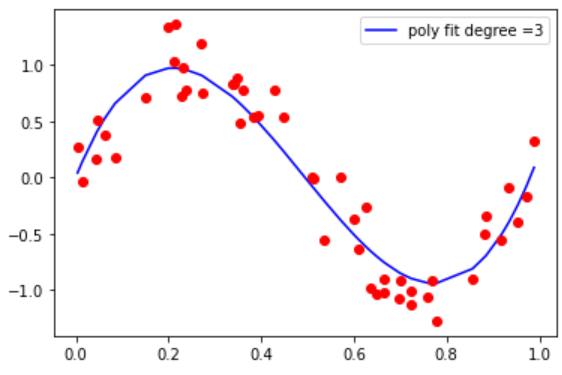
\includegraphics{images/Poly reg.png}
    \end{center}
\end{itemize}
\textbf{Bias-Variance Tradeoff:}
The learning goal is to find the best tradeoff between bias and variance.
\begin{itemize}
    \item The \textbf{bias} error is produced by weak assumptions in the learning algorithm. High bias can cause an algorithm to miss relevant relations between features and target outputs (\textbf{underfitting}).
    \item The \textbf{variance} is an error produced by an over-sensitivity to small fluctuations in the training set. High variance can cause an algorithm to model the random noise in the training data, rather than the intended outputs (\textbf{overfitting}).
    \begin{center}
        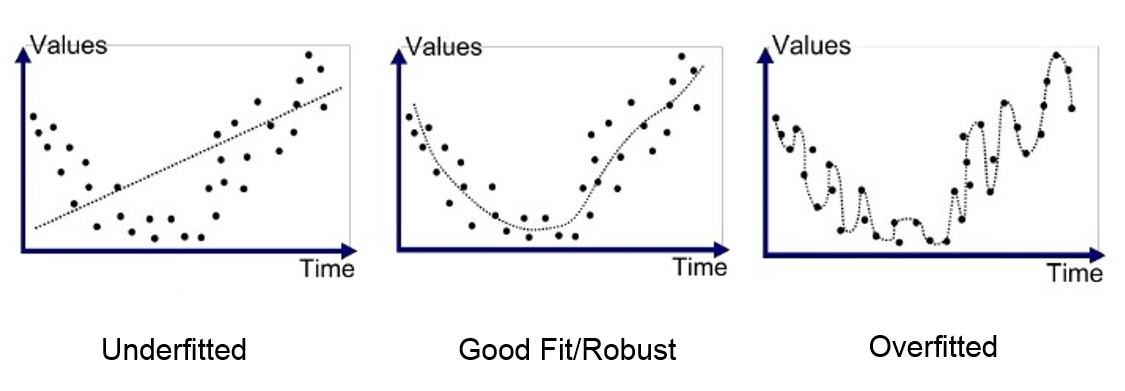
\includegraphics[scale = 0.35]{images/Overfitting vs Underfitting.png}
    \end{center}
\end{itemize}
\end{itemize}


\chapter{Machine Learning Basics II}
\section{Linear Regression}
Notation
\begin{itemize}
    \item m = Number of training examples
    \item x's = "input" variables/features
    \item y's = "output" variable/target variable
    \item $\{(x^{(i)},y^{(i)})\}$ = Training set
    \begin{flushleft}
        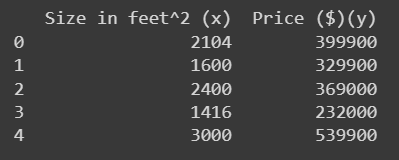
\includegraphics[scale = 0.7]{images/Training set.png}
    \end{flushleft}
    \item $h_{\theta}(x)$ = Hypothesis
\end{itemize}
Given a function $h_{\theta}(x)$ (e.g. $h_{\theta}(x) = \theta_{0} + \theta_{1}x$), choose $\theta_{0} \theta_{1}$ so that $h_{\theta}(x)$ is closed to $y$ in our training set $\{(x^{(i)},y^{(i)})\}$.
\begin{center}
    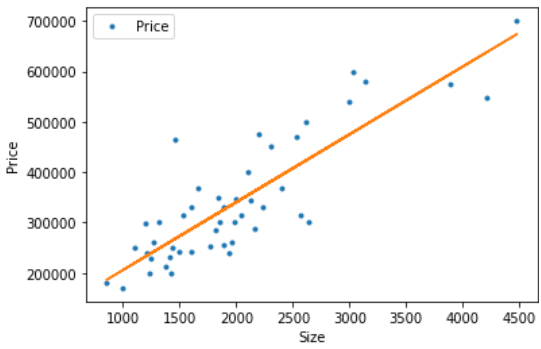
\includegraphics{images/Linear Ref.png}
\end{center}
To do that, we need to define a measure of the committed error, a \textbf{cost function} $J(\theta_{0},\theta_{1})$.
The goal is to find $\theta_{0} \theta_{1}$ in order to minimize $J(\theta_{0},\theta_{1})$ (e.g sum of square distances).
\[minimize_{\theta_{0} \theta_{1}}\frac{1}{2m}\sum_{i = 1}^{m}(h_{\theta}(x^{(i)}) - y^{(i)})^{2}\]

\subsection{Example with only one parameter}
Let's consider a simple example of linear regression with a function $h_{\theta}(x) = \theta_{1}x$ and a cost function $J(\theta_{1}) = \frac{1}{2m}\sum_{i = 1}^{m}(h_{\theta}(x^{(i)}) - y^{(i)})^{2}$.
\begin{center}
    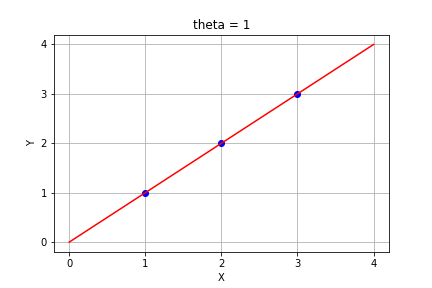
\includegraphics[scale = 0.7]{images/Simple liner reg.png}
\end{center}
As you can see from the graph above, our training set is composed by 3 points $\{(1,1), (2,2), (3,3)\}$. In this simple example the function $h_{\theta}(x)$ that perfectly fits the training set is the one with the parameter $\theta_{1} = 1$. In fact, if we compute the cost function $J(\theta_{1})$ with respect to $\theta_{1} = 1$, the result is 0 (minimized).
\[J(\theta_{1}) = \frac{1}{2m}\sum_{i = 1}^{m}(h_{\theta}(x^{(i)}) - y^{(i)})^{2}\]
\[= \frac{1}{2m}\sum_{i = 1}^{m}(\theta_{1}x^{(i)} - y^{(i)})^{2}\]
\[= \frac{1}{2m}(0+0+0)^2 = 0\]
But let's see what happens for different values of $\theta_{1}$.
\begin{itemize}
    \item $\theta_{1} = \frac{1}{2}$ $J(\theta_{1}) \approx 0.67$
    \item $\theta_{1} = 0$ $J(\theta_{1}) \approx 2.33$
    \item $\theta_{1} = -\frac{1}{2}$ $J(\theta_{1}) \approx 5.25$
\end{itemize}
\begin{center}
    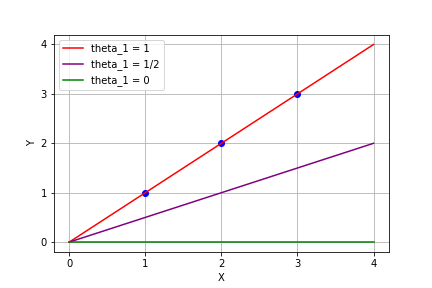
\includegraphics[scale = 0.7]{images/Simple liner reg (colors).png}
\end{center}
Now we can plot the values of $\theta_{1}$ on the \textbf{X} axis and the values of $J(\theta_{1})$ on the \textbf{Y} axis. The shape of $J(\theta_{1})$ will be the following:
\begin{figure}[h]
    \centering
    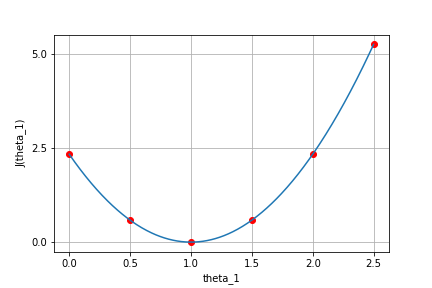
\includegraphics[scale = 0.7]{images/J.png}
    \label{Fig 1}
    \caption{Cost function J}
\end{figure}\newline
We obtain this \textbf{convex} function that has its minimum, for these specific $h_{\theta_{1}}(x^{(i)})$ and $y^{i}$, in 0. This principle is also valid for $n$-dimensional functions but the graphic representation is not that easy.\newline
How can we find $\theta_{1}$ in an automatic way?
\subsection{Gradient descent}
\textbf{Derivative:}\newline
The derivative tells us the slope of a function at any point. Given a point:
\begin{itemize}
    \item Positive derivative means that the function increases at that point
    \item Negative derivative means that the function decreases at that point.
    \item Null derivative means that there is a stationary point (minimum, maximum or saddle point).
\end{itemize}
Starting from a random configuration of $\theta$, each parameter is updated in the following way:
\[\theta_{k+1} = \theta_{k} - \eta \nabla J(\theta_{k})\]
where: 
\begin{itemize}
    \item $\nabla J(\theta_{k})$ is the partial derivative of the cost function in $\theta_{k}$.
    \item $\theta = \{\theta_{0},...,\theta_{n}\}$
    \item The parameter $\eta > 0$ is known as the \textit{learning rate}. 
\end{itemize}
Let's consider again the previous example with hypothesis function $h_{\theta}(x) = \theta_{1}x$. Our goal is to apply gradient descent algorithm in order to find a value of $\theta_{1}$ in which the partial derivative of $J$ is 0 where the function has a local minimum (so the cost function is minimized). For our simple example that point is $\theta_{1} = 1$\newline
Given the expression: 
\[\theta_{1} := \theta_{1} - \eta \frac{\partial}{\partial \theta_{1}}J(\theta_{1})\]
The derivative term $\frac{\partial}{\partial \theta_{1}}J(\theta_{1})$ can be:
\begin{itemize}
    \item $\geq 0$ it means that the function is increasing, so we are decreasing $\theta_{1}$ in the \textit{right direction}.
    \item $\leq 0$ it means that the function is decreasing, so we are increasing $\theta_{1}$ in the \textit{right direction}
\end{itemize}
\begin{flushleft}
    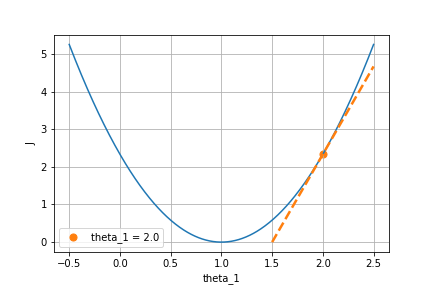
\includegraphics[scale=0.5]{images/partial derivative.png}
    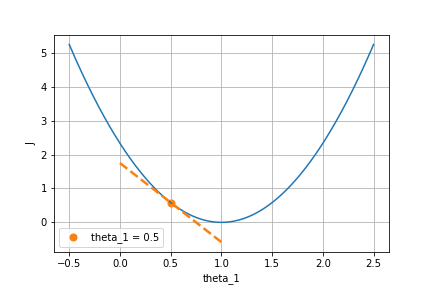
\includegraphics[scale=0.5]{images/partial derivative_1.png}
\end{flushleft}
\begin{center}
    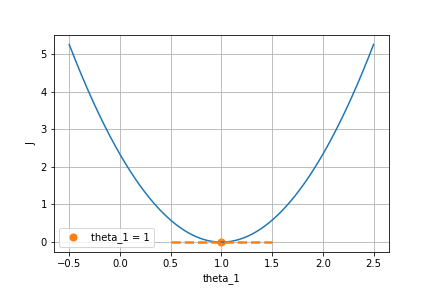
\includegraphics[scale=0.5]{images/partial derivative_2.png}
\end{center}
if $\eta$ is too small, gradient descent can be slow. Anyway, if it is too large, it can overshoot the minimum (fail to converge).\newline
The partial derivative of the cost function used in the previous example is the following:
\[\frac{\partial}{\partial \theta_{1}} \frac{1}{2m}\sum_{i=1}^{m}(\theta_{1}x^{(i)} - y^{(i)})^{2}\]
\[= \frac{1}{m}\sum_{i=1}^{m}(\theta_{1}x^{(i)} - y^{(i)})x^{(i)}\]
The algorithm also works with an n-dimensional input (multiple parameters $\theta$).
There are different ways in which the algorithm can be applied:
\begin{itemize}
    \item \textbf{Batch gradient descent:} Each step of gradient descent uses all training examples.
    \item \textbf{Stochastic gradient descent:} Update the parameters for each training case in turn, according to its own gradients.
    \item \textbf{Mini-batch gradient descent}: Update the parameters using a subset of the sample.
\end{itemize}
\subsection{Binary Classification}
\textbf{Classification: } determine to which discrete category a specific example belongs to
\begin{itemize}
    \item Binary classification: Two possible labels
    \item Multi-class classification: multiple possible labels
\end{itemize}
We can perform binary classification using the Linear Regression technique seen before. What we have to do is to choose a \textit{Decision rule}.
Let's assume that we have two labels for our classes $Y \equiv \{(-1,+1)\}$. The decision rule could be $y = sign(h_{\theta}(x))$:
\begin{itemize}
    \item if $h_{\theta}(x) \geq 0$, predict $y=1$
    \item if $h_{\theta}(x) < 0$, predict $y=-1$
\end{itemize}
If we have $Y \equiv \{(0,+1)\}$ the decision rule could be instead:
\begin{itemize}
    \item if $h_{\theta}(x) \geq 0.5$, predict $y=1$
    \item if $h_{\theta}(x) < 0.5$, predict $y=0$
\end{itemize}
This specifies a \textit{linear classifier}. It has a linear boundary (hyperplane) which separates the space.
\begin{center}
    \includegraphics[scale = 0.7]{images/Hyperplanes in R^2.png}
\end{center}
In 2D it is a line, in 3D is a plane and so on.\newline
Applying linear regression to classification tasks is not always a great idea since it is very influenced by outliers.
\section{Logistic Regression}
Although the term regression appears in its name, logistic regression is a classification algorithm.
The hypothesis space is composed by functions of type:
\[h_{\theta}(x) = g(\theta^{T},x) = \frac{1}{1 + e^{-\theta^{T}x}}\]
where $g(z) = \frac{1}{1 + e^{-z}}$ is the sigmoid/logistic function.\newline
\textbf{Example:} $h_{\theta}(x) = \frac{1}{1 + e^{-(\theta_{0} + \theta_{1}x)}}$
\begin{figure}[h]
    \centering    
    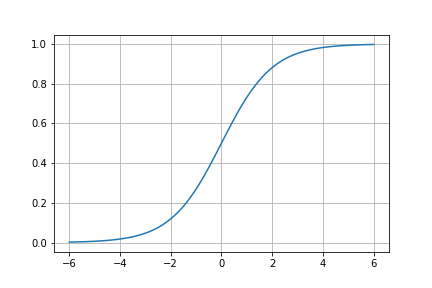
\includegraphics[scale=0.5]{images/sigmoid.png}
    \caption{$\theta_{0} = 0$, $\theta_{1} = 1$}
    \label{fig:sigmoid}
\end{figure}
\begin{figure}[h]
    \centering
    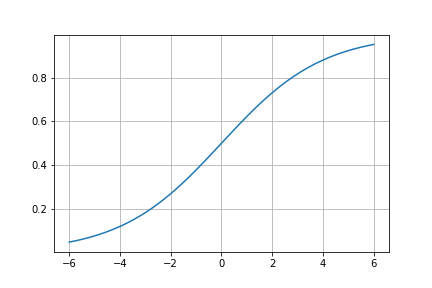
\includegraphics[scale=0.5]{images/sigmoid_1.png}
    \caption{$\theta_{0} = 0$, $\theta_{1} = 1$}
    \label{fig:sigmoid_1}
\end{figure} \newline
Note that $\theta_{0}$ and $\theta_{1}$ determine the shape of the function.\newline
As in the case of Linear regression, we have to choose a \textit{Decision rule}. Suppose to predict: 
\begin{itemize}
    \item $y = 1$ if $h_{\theta}(x) \geq 0.5$
    \item $y = 0$ if $h_{\theta}(x) < 0.5$ 
\end{itemize}
So, although the sigmoid function is a non-linear function, Logistic regression is still a linear model because the \textbf{decision boundary} is linear. One of the advantages of using Logistic regression is that is more robust with respect to \textit{outliers}
\begin{center}
    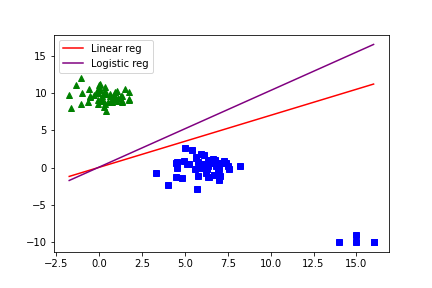
\includegraphics[scale=0.7]{images/linear vs log.png}
\end{center}
Finally, The cost function defined for logistic regression is not Mean Square Error. This is because it is no more a \textbf{convex} function when $h_{\theta}(x) = \frac{1}{1 + e^{-\theta^{T}x}}$. So, in order to optimize gradient descent algorithm, we will use \textbf{Cross-Entropy Cost Function}: $J(\theta) = \frac{1}{m} \sum_{i = 1}^{m}cost(h_{\theta}(x^{(i)}), y^{(i)})$ \newline
where $cost(h_{\theta}(x^{(i)}), y^{(i)})$ = 
\[
    \begin{cases}
         - \log(h_{\theta}(x^{(i)}))  & y^{(i)} = 1\\
         - \log(1 - h_{\theta}(x^{(i)})) & y^{(i)} = 0
    \end{cases}
\]
Simplified notation:
\[J(\theta) = - \frac{1}{m}\sum_{i=1}^{m}( y^{(i)} \cdot \log(h_{\theta}(x^{(i)})) + (1 - y^{(i)}) \cdot \log(1 - h_{\theta}(x^{(i)}))  )\]
This is a \textbf{convex} function, so we can use the gradient descent update rule mentioned before \footnote{Note that even with Mean Square error cost function we could have used gradient descent algorithm, but the derivative of $J(\theta)$ would have been different}:
\[\theta_{j} := \theta_{j} - \eta \frac{\partial}{\partial \theta_{j}}J(\theta) = \theta_{j} - \frac{\eta}{m}\sum_{i=1}^{m}(h_{\theta}(x^{(i)}) - y^{(i)})x_{j}\]


\chapter{Filters I}

\section{Image representation}
An \textbf{image} is a spatial distribution (two- or three-dimensional) of a physical entity that contains information related to the object (scene) that the image represents. That distribution can be represented as a continuous function that associates, to each point in the plane/space, the intensity of the physical entity at that point $f : \mathbb{R}^{2} \rightarrow \mathbb{R}$(or $f : \mathbb{R}^{3} \rightarrow \mathbb{R}$ for three-dimensional images).\newline
\textbf{Example:}\newline
Let's consider a monochrome image expressible by a continuous function with two independent variables:
\[f(n,m), f: \mathbb{R} \times \mathbb{R} \rightarrow \mathbb{R}\]
\begin{itemize}
    \item \textit{n, m} are the independent spatial coordinates of the image plane
    \item $f(n,m)$ gives the intensities of the measured physical quantity (usually light) at position ($n,m$).
\end{itemize}

\subsection{Digitization}
For digital processing is required a discrete representation of the images. This discretization process is composed by:
\begin{itemize}
    \item \textbf{sampling:} can be expressed as a partition of the image plane in a grid of cells.
    \item \textbf{quantisation:} conversion from the continuous range of values of image intensity to a discrete and finite set of grey values [0-255].
\end{itemize}
\subsection{Digital image representation}
Images can be seen as a Cartesian coordinates system.
\[
    f[n,m] = 
    \begin{bmatrix}
    \ddots & \vdots & \vdots& \vdots & \\
    \dots & f[-1,1] & f[0,1] & f[1,1] & \dots\\
    \dots & f[-1,0] & f[0,0] & f[1,0] & \dots\\
    \dots & f[-1,-1] & f[0,-1] & f[1,-1] &\dots\\
     & \vdots & \vdots & \vdots & \ddots\\
    \end{bmatrix}
\]
where $f[n,m]$ is a \textbf{discrete} function and $n,m$ correspond to rows and columns of a matrix. Each element of the matrix is a \textbf{pixel} and each pixel can have a value, in case of  a grey scale image, between 0-255. By convention, $f[0,0]$ is the center of the image.

\section{Colors}
\subsection{RGB representation}
\begin{center}
    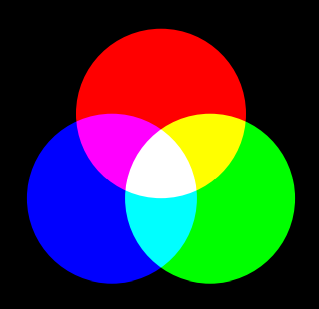
\includegraphics{images/RGB.png}
\end{center}
In the RGB (Red, Green, Blue) system, the primary colors are:
\begin{itemize}
    \item red
    \item green
    \item blue
\end{itemize}
By composing two primary colors, you obtain secondary colors:
\begin{itemize}
    \item cyan = green + blue
    \item magenta = red + blue
    \item yellow = red + green
\end{itemize}
By composing all the primary colors, you obtain white.\newline
An RGB-encoded image consists of three channels, one for each component, where each color is obtained mixing red, green and blue values. If you use 8 bit to represent each component, the number of distinct colors that can be represented in the image is $(2^{8})^{3} = 16 777 219$.\newline
The function that describes an RGB-image is the following:
$$f[n,m] = \left[
\begin{array}{c}
r[n,m]\\
g[n,m]\\
b[n,m]
\end{array}\right]
$$

\subsection{HSV representation}
\begin{center}
    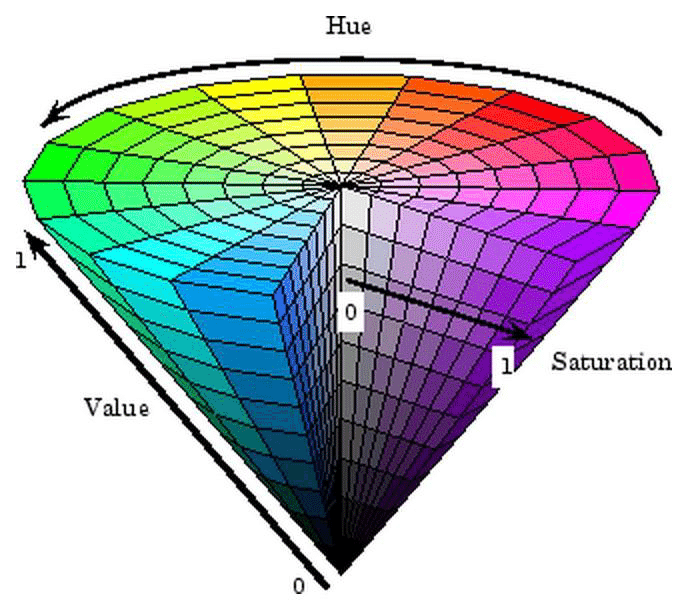
\includegraphics[scale = 0.3]{images/HSV.png}
\end{center}
The HSV representation specifies colors in term of:
\begin{itemize}
    \item \textbf{hue:} dominant color
    \item \textbf{saturation:} it measures how far you are from the fully saturated color (in which you don't have any grey).
    \item \textbf{lightness:} color brightness. While saturation measures the “dilution” of hue with white, brightness indicates dilution with black.
\end{itemize}
HSV representation is closer to how people perceive colors.

\section{Histogram of an image}
The histogram of an image associates to each grey (or RGB) level the number of pixels in which it occurs (i.e. its frequency). So it represents the global distribution of grey (or RGB) levels in a given image.
\begin{flushleft}
    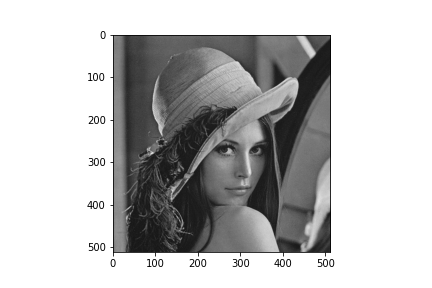
\includegraphics[scale=0.5]{images/lena GS.png}
    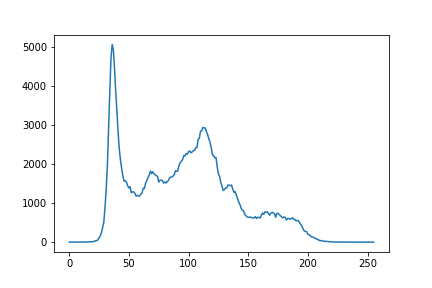
\includegraphics[scale=0.5]{images/histogram GS.png}
    
    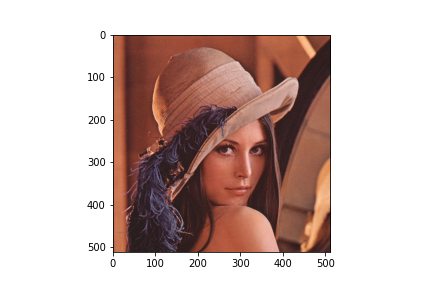
\includegraphics[scale=0.5]{images/lena RGB.png}
    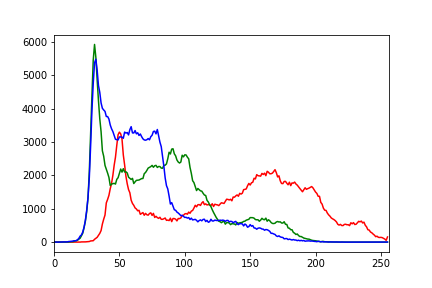
\includegraphics[scale=0.5]{images/histrogram RGB.png}
\end{flushleft}
Histograms are very simple image representation and they are not robust at all against any image transformation (e.g. changing in illumination).

\section{Filters}
\textbf{Filtering:} Forming a new image whose pixel values are transformed from the original ones.\newline
The goals of filtering are:
\begin{itemize}
    \item \textbf{extract} useful information
    \item \textbf{transform} images into another domain where we can modify/enhance image properties.
\end{itemize}
\subsection{Linear Filters}
We define a filter as a unit that converts an input function $f[n,m]$ into an output function $g[n,m]$, where ($n,m$) are the independent variables. \newline
Linear filters work by moving a sliding window (kernel) through the image, pixel by pixel. The window contains coefficients which characterize the transformation. At each position, the result of the filter is calculated by combining the values of the image subtended to the window with the coefficients of the window itself. In order to compute the new value of the central pixel, the coefficients are:
\begin{itemize}
    \item multiplied by the values of the original image subtended to the window
    \item added
\end{itemize}
These filters are defined by the following mathematical operator called \textbf{convolution}:
\[(f * h)[n,m] = \sum_{k,l}f[k,l]h[n-k, m-l]\]
where $h$ is the \textit{kernel}.\newline
Note that the kernel must have an odd number of rows and columns, because it is centered on the pixel to process.\newline \newline
\textbf{Borders:}\newline
Given an $n \times n$ kernel, its external row/column coincides with the border of the image when the center of this mask is at distance $\frac{n-1}{2}$ from the edge. If you move further out, part of the window \textit{leaves} the image.\newline
This situation can be managed in three different ways:
\begin{itemize}
    \item limit the movement of the mask, keeping it at a minimum distance of $\frac{n-1}{2}$ from the edges.
    \item duplicate the external rows/columns of the image
    \item enlarge the image with rows/columns of zeros
\end{itemize}
Solution 1 gives reliable results, but produces a different size image from the original. Solutions 2 and 3, on the other hand, give results that are not exactly authentic near the edges, but are often convenient because they allow you to obtain an output image with the same size as the input one.

\subsection{Smoothing filters}
Smoothing filters are low-pass filters: they emphasize low frequencies and attenuate the high frequencies. They cause image blur, which is helpful to:
\begin{itemize}
    \item remove small details
    \item reduce noise in the image
\end{itemize}
\textbf{Examples:}
\begin{itemize}
    \item \textbf{Moving average filter} (\textit{box filter}) in which all the kernel coefficients are equal to 1.
    \begin{center}
        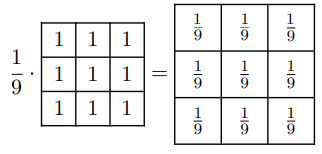
\includegraphics[]{images/box filter.png}
    \end{center}
    It is defined by the following formula:
    \[g[n,m] = \frac{1}{9}\sum_{k=-1}^{1}\sum_{l=-1}^{1}f[n-k, m-l]\]
    Basically, it replaces each pixel with an average of its neighbors. This filter can be applied in order to remove small details, to obtain blurring effect (more evident as the size of the window increases) but it is not useful to remove the so called \textit{salt and pepper noise}, because corrupted pixels affect the computation of the average, so the noise points can even tend to dilate.
    
    \item \textbf{Gaussian Filter} is a weighted average filter with coefficients derived from two-dimensional Gaussian function.
    \begin{center}
        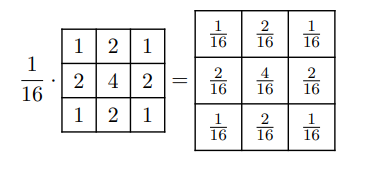
\includegraphics[]{images/gaussian filter.png}
    \end{center}
    where 16 is the sum of the kernel coefficients\newline
    The one-dimensional Gaussian with mean $\mu$ and standard deviation $\sigma$ has the following shape:
    \[G(x) = \frac{1}{\sigma \sqrt{2\pi}}e^{-\frac{(x-\mu)^{2}}{2\sigma^{2}}}\]
    \begin{center}
        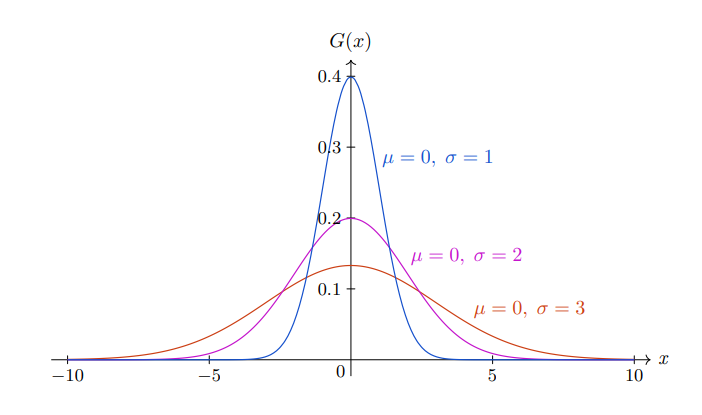
\includegraphics[]{images/Gaussian.png}
    \end{center}
    The kernel is an approximation of a 2D Gaussian function in which pixels near the center of the window have more weight than the outer ones
    \[\frac{1}{2\pi \sigma^{2}}e^{-\frac{u^{2} + v^{2}}{2\sigma^{2}}}\]
    Like the box-filter presented above, it removes high-frequency components and produces blurring effect.\newline\newline
    The filter has two main parameters:
    \begin{itemize}
        \item \textbf{size of the kernel}: A bigger kernel approximates better the Gaussian function, but it increases the computational cost of the filtering process
        \item \textbf{variance} $\sigma$: It determines the extent of smoothing. Increasing the value of $\sigma$ means to increase the blurring effect. In fact, as sigma increases, the weights of the pixels near the center decrease and the weights of the outer pixels increase.
    \end{itemize}
\end{itemize}
Note that, for this kind of filters, the sum of the window's values has to be equal to one, because constant regions shouldn't be affected by the application of the filter
\subsection{Median filter}
The median filter is not a convolutive operator. In fact, it uses an "empty" window, with no coefficients: it replaces each pixel of the input image with the \textbf{median} of its neighborhood. This filter is effective in reducing \textit{salt and pepper noise}, because the presence of any corrupted pixel does not influence the result (unless these pixels are particularly numerous in a certain neighbourhood). Also, it does not degrade too much the edges of the image.


\chapter{Filters II}

\section{More on convolution}
\begin{itemize}
    \item \textbf{Convolution}: $(f * h)[n,m] = \sum_{k,l}f[k,l] h[n-k, m-l]$
    \item \textbf{Cross-correlation}: $(f$ \ding{72} $h)[n,m] = \sum_{k,l}f[k,l] h[n+k, m+l]$
\end{itemize}
The only difference between the two is the way the kernel is applied. In fact, a convolutive operator applies a flipped version, in both dimension, of the sliding window.
\begin{center}
    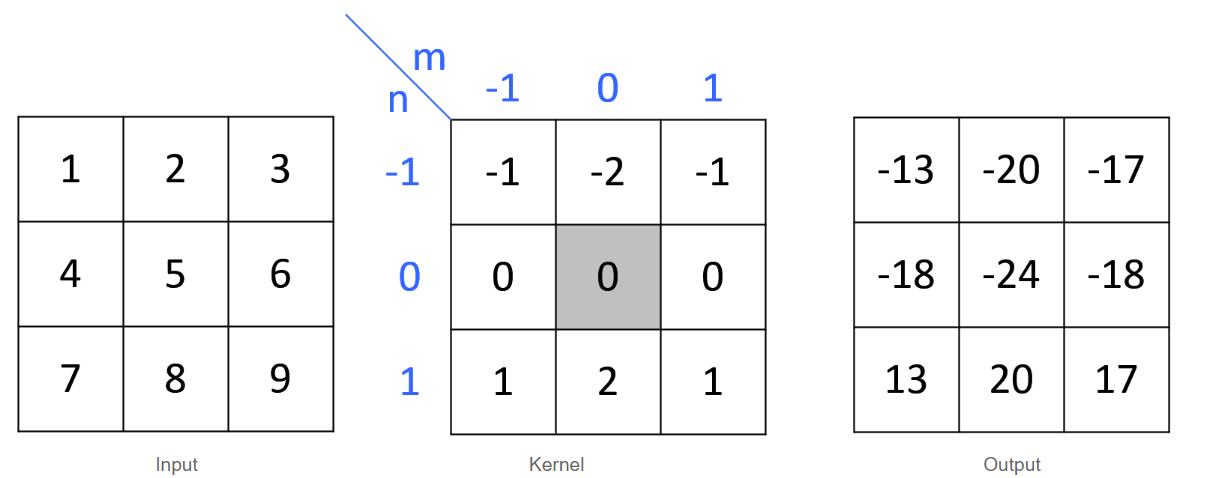
\includegraphics[scale =0.5]{images/flipped kernel.png}
\end{center}
more details here: \url{ http://www.songho.ca/dsp/convolution/convolution2d_example.html}

\subsection{Properties of convolution}
\begin{itemize}
    \item \textbf{Commutative}: $(f * g) = (g * f)$
    \item \textbf{Associative}: $(f * g) * h = f * (g * h)$
    \item \textbf{Homogeneity}: $\textbf{k}f*g = f*\textbf{k}g = \textbf{k}(f*g)$
    \item \textbf{Distributive}: $f * (g + h) = (f * g) + (f * h)$
    \item \textbf{Shift invariant}: Operator behaves the same everywhere, i.e. the value of the output depends on the pattern in the image neighborhood, not on the position of the neighborhood
    \item \textbf{Separability}: 2D convolution is separable, and we can factor into two steps (i.e. first convolve all rows with a 1D filter, then convolve all columns with a 1D filter).
\end{itemize}

\section{Sharpening filters}
A sharpening filter emphasizes image details. They are high pass filters that emphasize high frequencies, and penalize low frequencies.\newline
The sharpening effect is obtained in two steps:
\begin{itemize}
    \item Apply an operator that extracts the details of the image (produces an image with light values in the transition areas and dark values in the uniform areas)
    \item This result is added to the original image
\end{itemize}
One way to obtain the details is by applying a smoothing filter to an image and computing a pixel by pixel difference between the original image and the smoothed one. Then you add the resulting image to the original one to obtain the sharpening effect.
\begin{flushleft}
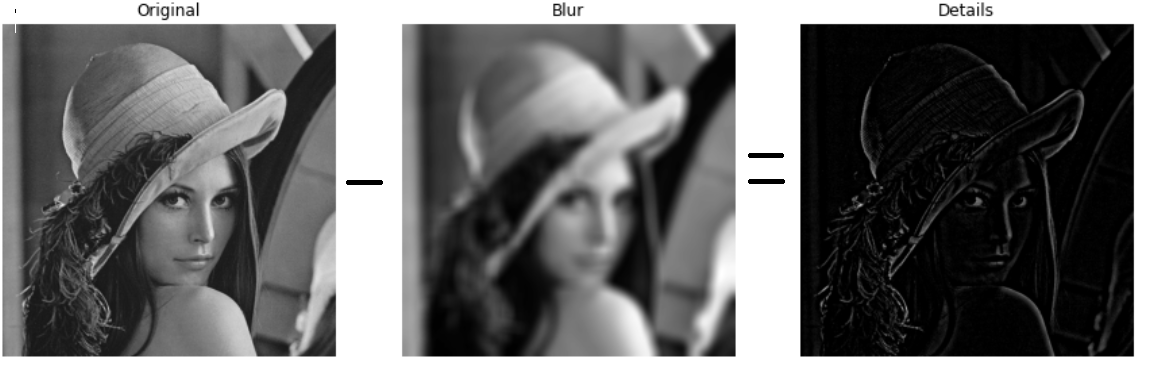
\includegraphics[scale=0.6]{images/details.png}
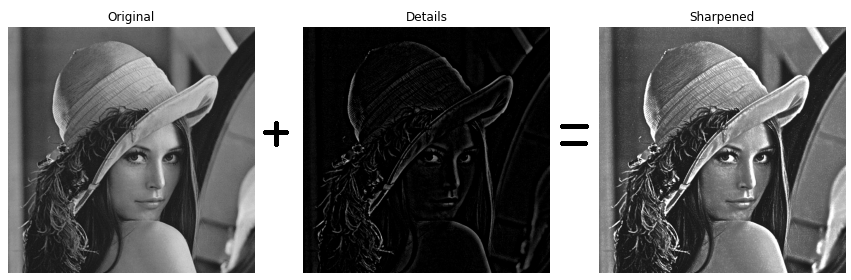
\includegraphics[scale = 0.8]{images/Lena sharpened.png}
\end{flushleft}
\section{Edge detection}
An edge is a set of connected pixels between two regions in which there is a sudden change in intensity. These discontinuities can be caused by:
\begin{itemize}
    \item Illumination discontinuity: cast shadows
    \item Change in surface orientation: shape
    \item Depth discontinuity: object boundary
    \item Surface color discontinuity
\end{itemize}
The goal of edge detection is to detect easily and automatically these regions.\newline
Basically, a simple edge detection algorithm computes the first order derivative of the intensity function of an image and detects as edges the extremes of the derivative function.
\begin{flushleft}
    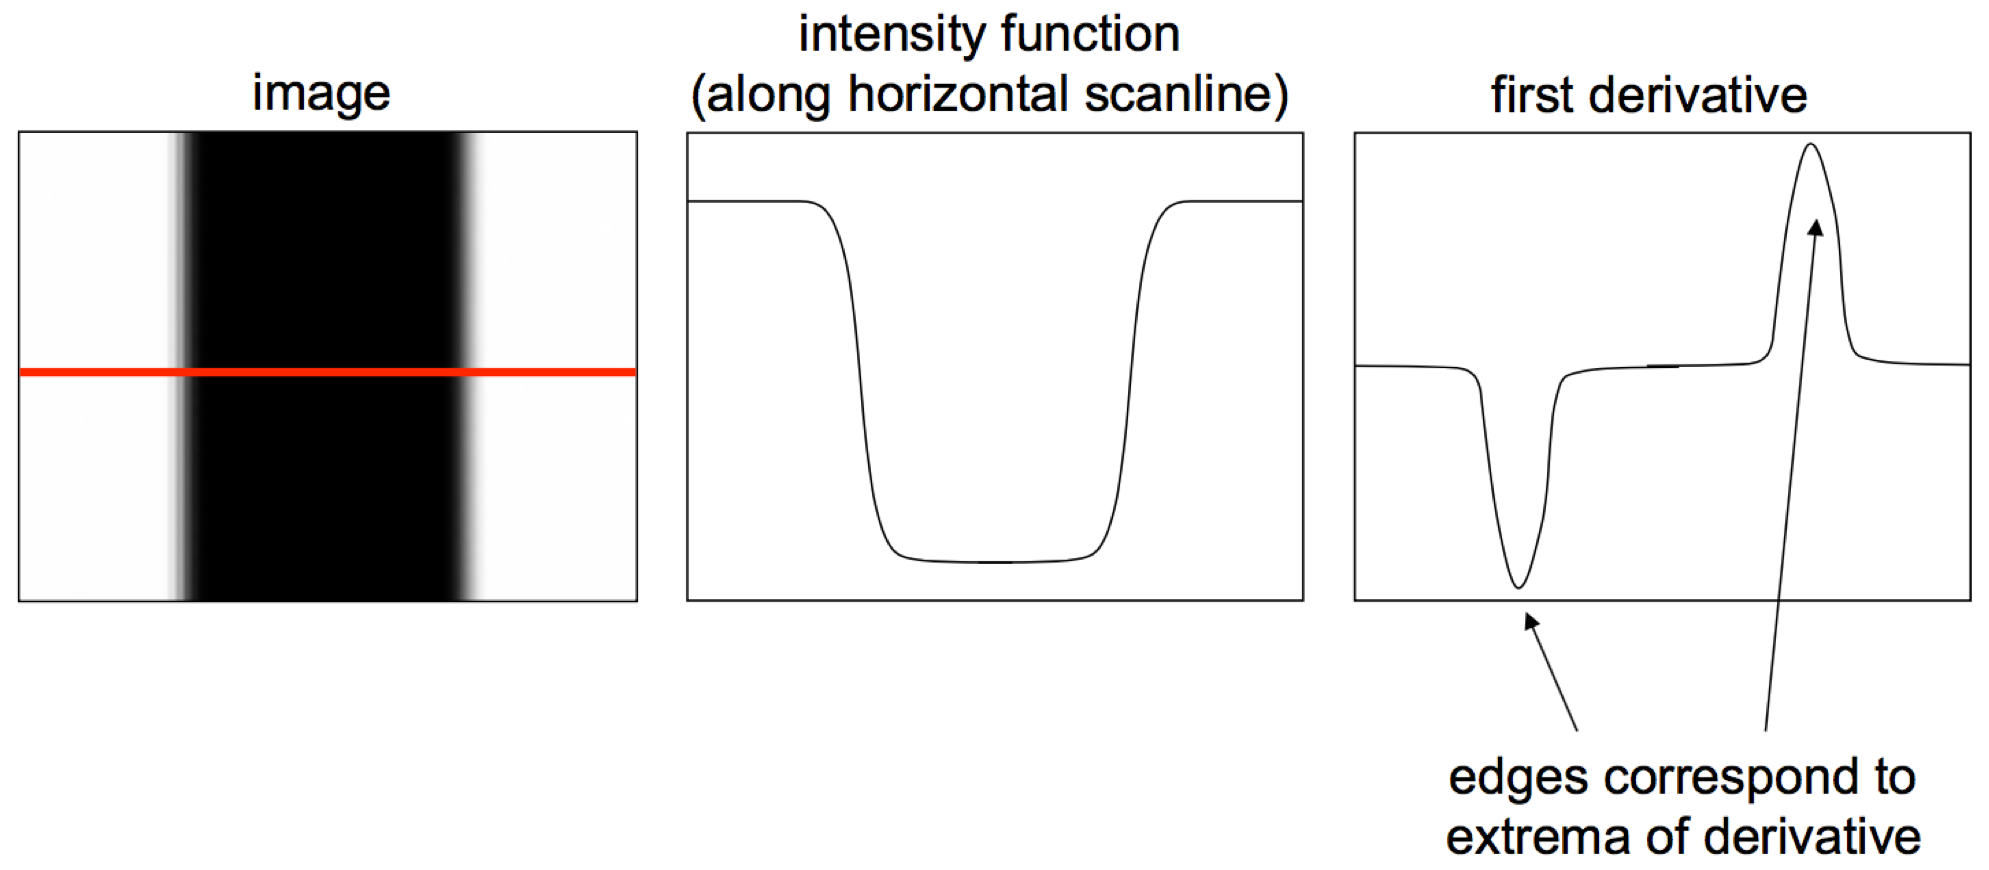
\includegraphics[scale = 0.4]{images/edge detection.png}
\end{flushleft}
\subsection{Discrete approximation of the derivatives}
In order to apply a derivative operator in a digital environment, we need a discrete approximation of derivatives. 
\begin{itemize}
    \item Derivative in 1D:
    \[\frac{df}{dx} = lim_{\Delta x \rightarrow 0} \frac{f(x) - f(x - \Delta x)}{\Delta x} = f^{'}(x)\]
    \item Discrete derivative in 1D:
    \[\frac{df}{dx} = lim_{\Delta x \rightarrow 0} \frac{f(x) - f(x - \Delta x)}{\Delta x} = f^{'}(x)\]
    \[= \frac{f(x) - f(x - 1)}{1} = f^{'}(x)\]
    \[= f(x) - f(x - 1) = f^{'}(x)\]
\end{itemize}
Operators based on the first order derivative must satisfy the following properties:
\begin{itemize}
    \item have zero value in the homogeneous sections of the image (no response in constant regions)
    \item have a non-zero value along the transition areas.
\end{itemize}
Formulations satisfying these properties can be defined in terms of differences between pixel values.
\begin{flushleft}
    \begin{tabular}{c | c | c}
     \textbf{Name} & \textbf{Discrete derivative} & \textbf{Filter}\\
     \hline\xrowht{20pt}
     Backward & $\frac{df}{dx} = f(x) - f(x-1)$ & [0 1 -1]  \\
     \xrowht{20pt}
     Forward & $\frac{df}{dx} = f(x) - f(x+1)$ & [-1 1 0]\\
     \xrowht{20pt}
     Central & $\frac{df}{dx} = f(x+1) - f(x-1)$ & [1 0 -1]
    \end{tabular}
\end{flushleft}
Note that each discrete approximation can be defined as an application of convolution using the respective 1D filter (the same is valid also for 2D images).\newline\newline\newline\newline\newline\newline
\textbf{Backward example:}
Backward derivative is obtained by computing the difference between the value of the current pixel and the value of the previous one.
\begin{flushleft}
    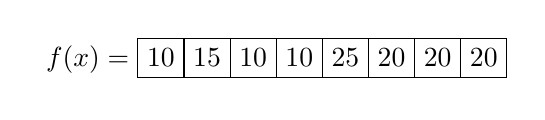
\begin{tikzpicture}
    \matrix[matrix of nodes, row 1 column 1/.style={nodes={draw=none, fill=none}},nodes={minimum size=0.5cm, draw}, row sep=-\pgflinewidth, column sep=-\pgflinewidth](mygrid){%
    $f(x) = $ & 10 & 15 & 10 & 10 & 25 & 20 & 20 & 20\\
    };
    \end{tikzpicture}
    
    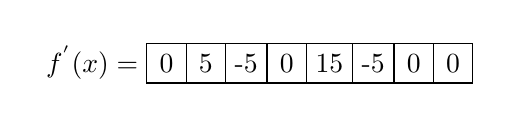
\begin{tikzpicture}
    \matrix[matrix of nodes, row 1 column 1/.style={nodes={draw=none, fill=none}},nodes={minimum size=0.5cm, draw}, row sep=-\pgflinewidth, column sep=-\pgflinewidth](mygrid2){%
    $f^{'}(x) = $ & 0 & 5 & -5 & 0 & 15 & -5 & 0 & 0\\
    };
    \end{tikzpicture}
\end{flushleft}
That is the same of applying convolution using the kernel [0 1 -1] (flipped).\newline \newline
According to this, a 2D derivative filter could be defined by the following kernels (central derivative):
\begin{figure}[h]
        \centering
        \begin{minipage}{0.45\linewidth}
        \centering
        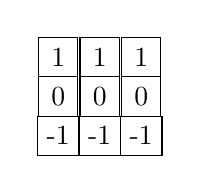
\begin{tikzpicture}
            \matrix[matrix of nodes ,nodes={minimum size=0.5cm, draw}, row sep=-\pgflinewidth, column sep=-\pgflinewidth](sobel_hz){%
            1 & 1 & 1\\
            0 & 0 & 0\\
            -1 & -1 & -1\\
            };
        \end{tikzpicture}
        \caption*{Detects horizontal edges}
        \end{minipage}
        \hspace{20pt}
        \begin{minipage}{0.45\linewidth}
        \centering
        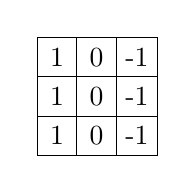
\begin{tikzpicture}
            \matrix[matrix of nodes ,nodes={minimum size=0.5cm, draw}, row sep=-\pgflinewidth, column sep=-\pgflinewidth](sobel_v){%
            1 & 0 & -1\\
            1 & 0 & -1\\
            1 & 0 & -1\\
            };
        \end{tikzpicture} 
        \caption*{Detects vertical edges}
        \end{minipage}
\end{figure}

\subsection{Image gradient}
The operators based on the first order derivative are formulated starting from \textbf{gradient}. Given a function $f(x,y)$ (2D image), the gradient vector is defined as follows:
\[
    \nabla f = 
    \begin{bmatrix}
        G_{x}\\
        G_{y}\\
    \end{bmatrix}
    =
    \begin{bmatrix}
        \frac{\partial f}{\partial x}\\
        \vspace{1pt}\\
        \frac{\partial f}{\partial y}\\
    \end{bmatrix}
\]
The image gradient is obtained by applying two-dimensional derivative filters and it provides the following information:
\begin{itemize}
    \item The partial derivatives with respect to both horizontal and vertical directions.
    \item The gradient magnitude, which indicates the intensity of the discontinuity.
    \[|| \nabla f || = \sqrt{G_{x}^{2} + G_{y}^{2}}\]
    \item The gradient direction, given by:
    \[ \theta = tan^{-1} \left (\frac{G_{y}}{G_{x}} \right)\]
    \item It points in the direction of most rapid increase in intensity.
\end{itemize}
\begin{center}
    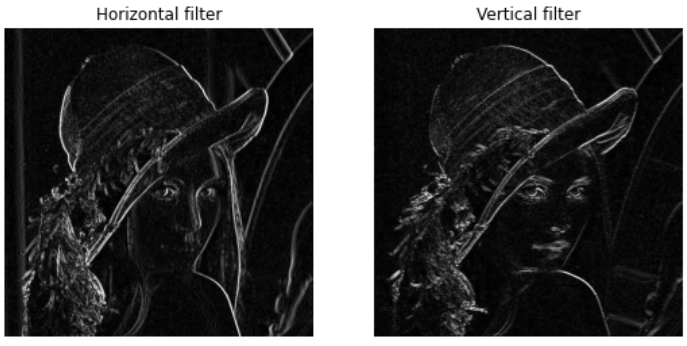
\includegraphics[scale = 0.8]{images/lena hx hy.png}
\end{center}
\subsection{Effects of noise}
Derivative operators are sensitive to noise. Thus, it may be impossible to detect edges of a noisy image (even if the noise is not so strong).
In these cases it is useful to perform a smoothing operation before applying the derivative filter.\newline
For example, we can look for peaks in $\frac{d}{dx}(f * g)$ where $g$ is a smoothing kernel (e.g. Gaussian filter). By applying the differential property of convolution
\[\frac{d}{dx}(f * g) = f * \frac{d}{dx}g\]
which save us one operation. In fact, by doing this, you obtain a new filter $ \frac{d}{dx}g$ called \textbf{derivative of Gaussian} that performs at the same time both smoothing and derivative operation

\chapter{Local invariant features}
\section{Derivative of Gaussian filter}
A two-dimensional Gaussian function centered in 0 is obtained as a product of two Gaussians oriented along the $x$ and $y$ axes. Its formula is:
\[G_{\sigma}(x,y) = \frac{1}{2\pi\sigma^{2}}e^{-\frac{x^{2} + y^{2}}{2\sigma^{2}}}\]
\[= \left( \frac{1}{\sqrt{2\pi}\sigma}e^{-\frac{x^{2}}{2\sigma^{2}}}\right) 
    \left( \frac{1}{\sqrt{2\pi}\sigma}e^{-\frac{y^{2}}{2\sigma^{2}}}\right)\]
So you can compute the two-dimensional derivative of Gaussian filter with respect to both $x$ and $y$ directions and combine the output.

\begin{itemize}
    \item $f^{'}_{x}$ (derivative with respect to $x$):
    \[-\frac{x}{2\pi\sigma^4}e^{-\frac{x^2+y^2}{2\sigma^2}}\]
    \item $f^{'}_{y}$ (derivative with respect to $y$):
    \[-\frac{y}{2\pi\sigma^4}e^{-\frac{x^2+y^2}{2\sigma^2}}\]
\end{itemize}
Kernels are an approximation of these derivative functions
\begin{center}
    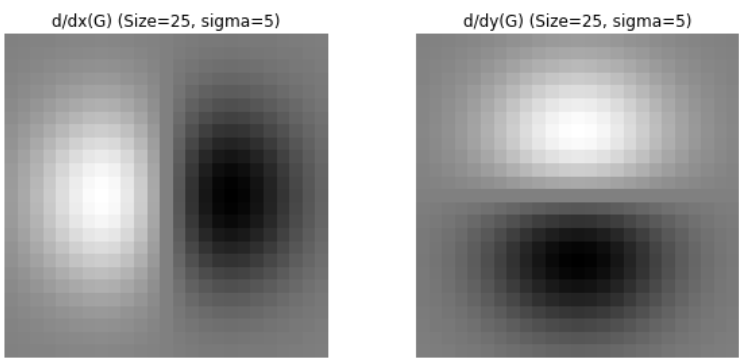
\includegraphics[scale = 0.6]{images/derivative gaussian.png}
\end{center}
Increasing the value of the parameter $\sigma$ means to apply a stronger smoothing effect (remove noise), but it will produce images with more blurred edges. With a low value of $\sigma$ we will be able to detect tiny edges, but with a weaker smoothing effect. This is the reason why $\sigma$ is usually referred as the \textbf{scale of the Gaussian derivative filter}.
\begin{itemize}
    \item Larger values: It detects larger scale edges
    \item Smaller values: It detects finer features
\end{itemize}
We can fine-tune $\sigma$ in order to detect edges at different scales. Basically, fine-tuning the scale could lead to detect edges that are either far \textit{from the camera} (very small) or near (larger).
\section{Examples of 2D derivative filters}
\begin{itemize}
    \item \textbf{Sobel filter:}
    Sobel filter is a derivative filter based on the derivative of Gaussian. It is defined by the following kernels:
    \begin{center}
        \begin{figure}[ht]
        \begin{minipage}{0.45\linewidth}
        \centering
        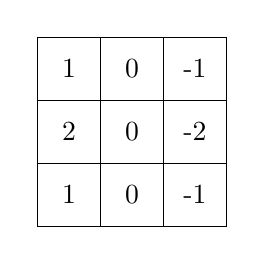
\begin{tikzpicture}
            \matrix[matrix of nodes ,nodes={minimum size=0.8cm, draw}, row sep=-\pgflinewidth, column sep=-\pgflinewidth](sobel_hz){%
            1 & 0 & -1\\
            2 & 0 & -2\\
            1 & 0 & -1\\
            };
        \end{tikzpicture}
        \caption*{Responds to vertical lines}
        \end{minipage}
        \hspace{20pt}
        \begin{minipage}{0.45\linewidth}
        \centering
        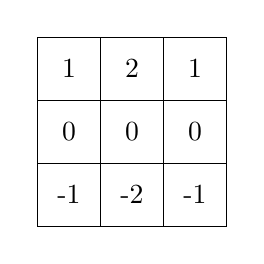
\begin{tikzpicture}
            \matrix[matrix of nodes ,nodes={minimum size=0.8cm, draw}, row sep=-\pgflinewidth, column sep=-\pgflinewidth](sobel_v){%
            1 & 2 & 1\\
            0 & 0 & 0\\
            -1 & -2 & -1\\
            };
        \end{tikzpicture} 
        \caption*{Responds to horizontal lines}
        \end{minipage}
    \end{figure}
    \end{center}
    Let's consider the filter that responds to vertical lines (the same is valid also for the other). It is made of two components.\newline \newline
    The first one is:
    \begin{flushleft}
        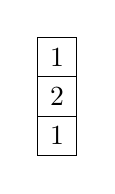
\begin{tikzpicture}
        \matrix[matrix of nodes ,nodes={minimum size=0.5cm, draw}, row sep=-\pgflinewidth, column sep=-\pgflinewidth](first_comp){%
        1\\
        2\\
        1\\
        };
        \end{tikzpicture}
    \end{flushleft}
    That is a 1D weighted average filter. \newline\newline 
    The second one is:
    \begin{flushleft}
        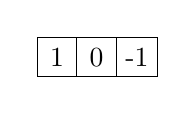
\begin{tikzpicture}
        \matrix[matrix of nodes ,nodes={minimum size=0.5cm, draw}, row sep=-\pgflinewidth, column sep=-\pgflinewidth](second_comp){%
        1 & 0 & -1\\
        };
        \end{tikzpicture}
    \end{flushleft}   
    That computes the 1D x-derivative according to the following discrete approximation (1D):
    \[\frac{df}{dx} = f(x+1) - f(x-1) = f^{'}(x)\]
    which is the \textit{central} derivative.\newline
    Thanks to the 1D weighted average component, this filter is less sensitive to noise. In fact, as the Gaussian filter does, it emphasizes pixels near the center of the kernel and has an averaging effect.
    \begin{center}
        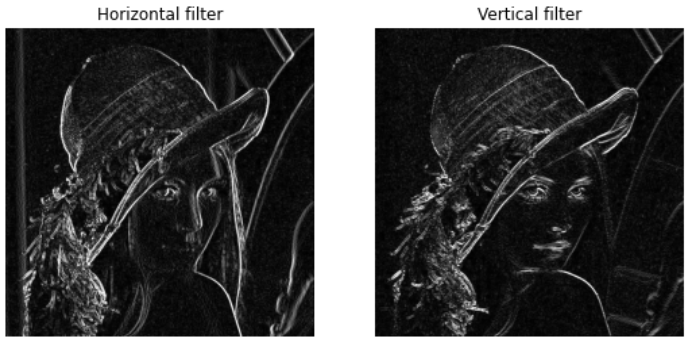
\includegraphics[scale = 0.7]{images/sobel lena.png}
    \end{center}
    \item \textbf{Prewitt filter:}
    Prewitt filter is a derivative filter similar to Sobel but less "sophisticated", because it doesn't have the weighted average component (it does not give more weight to pixels near the center).
    \begin{center}
        \begin{figure}[ht]
        \begin{minipage}{0.45\linewidth}
        \centering
        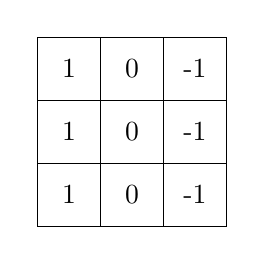
\begin{tikzpicture}
            \matrix[matrix of nodes ,nodes={minimum size=0.8cm, draw}, row sep=-\pgflinewidth, column sep=-\pgflinewidth](prewitt_hz){%
            1 & 0 & -1\\
            1 & 0 & -1\\
            1 & 0 & -1\\
            };
        \end{tikzpicture}
        \end{minipage}
        \hspace{5pt}
        \begin{minipage}{0.45\linewidth}
        \centering
        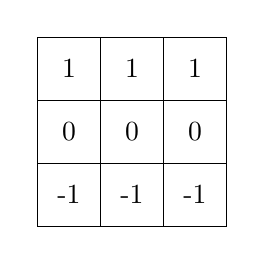
\begin{tikzpicture}
            \matrix[matrix of nodes ,nodes={minimum size=0.8cm, draw}, row sep=-\pgflinewidth, column sep=-\pgflinewidth](prewitt_v){%
            1 & 1 & 1\\
            0 & 0 & 0\\
            -1 & -1 & -1\\
            };
        \end{tikzpicture} 
        \end{minipage}
    \end{figure}
    \end{center}
    Let's see an application of this filter:
    \[
    I = 
    \begin{bmatrix}
        10 & 10 & 20 & 20 & 20\\
        10 & 10 & 20 & 20 & 20\\
        10 & 10 & 20 & 20 & 20\\
        10 & 10 & 20 & 20 & 20\\
        10 & 10 & 20 & 20 & 20\\
    \end{bmatrix}
    *\frac{1}{3}
    \begin{bmatrix}
       -1 & 0 & 1\\
       -1 & 0 & 1\\
       -1 & 0 & 1\\
    \end{bmatrix}
    =
    \begin{bmatrix}
       0 & 0 & 0 & 0 & 0\\
       0 & 10 & 10 & 0 & 0\\
       0 & 10 & 10 & 0 & 0\\
       0 & 10 & 10 & 0 & 0\\
       0 & 0 & 0 & 0 & 0\\
    \end{bmatrix}
    \]
    As you can see, it detects a vertical edge in the transition zone between 10 and 20.
    \item \textbf{Scharr filter:}
    Scharr filter is basically a Sobel operator in which central components are more emphasized.
    \begin{center}
        \begin{figure}[ht]
        \begin{minipage}{0.45\linewidth}
        \centering
        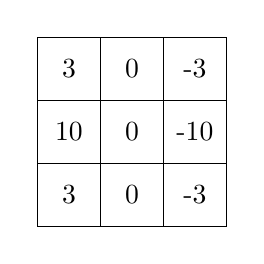
\begin{tikzpicture}
            \matrix[matrix of nodes ,nodes={minimum size=0.8cm, draw}, row sep=-\pgflinewidth, column sep=-\pgflinewidth](scharr_hz){%
            3 & 0 & -3\\
            10 & 0 & -10\\
            3 & 0 & -3\\
            };
        \end{tikzpicture}
        \end{minipage}
        \hspace{5pt}
        \begin{minipage}{0.45\linewidth}
        \centering
        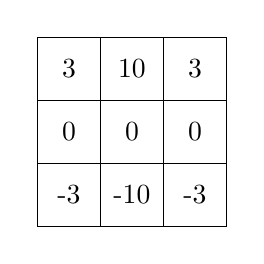
\begin{tikzpicture}
            \matrix[matrix of nodes ,nodes={minimum size=0.8cm, draw}, row sep=-\pgflinewidth, column sep=-\pgflinewidth](scharr_v){%
            3 & 10 & 3\\
            0 & 0 & 0\\
            -3 & -10 & -3\\
            };
        \end{tikzpicture} 
        \end{minipage}
    \end{figure}
    \end{center}
    \item \textbf{Roberts filter:} It considers diagonals.
    \begin{center}
        \begin{figure}[ht]
        \begin{minipage}{0.45\linewidth}
        \centering
        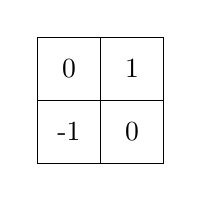
\begin{tikzpicture}
            \matrix[matrix of nodes ,nodes={minimum size=0.8cm, draw}, row sep=-\pgflinewidth, column sep=-\pgflinewidth](roberts_hz){%
            0 & 1\\
            -1 & 0\\
            };
        \end{tikzpicture}
        \end{minipage}
        \hspace{5pt}
        \begin{minipage}{0.45\linewidth}
        \centering
        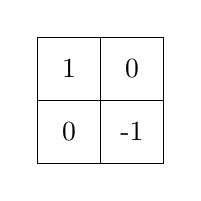
\begin{tikzpicture}
            \matrix[matrix of nodes ,nodes={minimum size=0.8cm, draw}, row sep=-\pgflinewidth, column sep=-\pgflinewidth](roberts_v){%
            1 & 0\\
            0 & -1\\
            };
        \end{tikzpicture} 
        \end{minipage}
    \end{figure}
    \end{center}
\end{itemize}
\section{Canny edge detector}
Canny algorithm is a 4-step edge detection method:
\begin{enumerate}
    \item Application of a Gaussian smoothing filter.
    \item Find magnitude and orientation of gradient by using a first order derivative filter.
    \item Non-maximum suppression: select single maximum, in terms of gradient magnitude, along the orthogonal direction to the edge (non-maximums are set to 0 and only maximums are kept).
    \item Selection of significant edges by \textit{hysteresis} thresholding, which is based (usually) on two thresholds, $T1$ and $T2$, with $T1 > T2$:
    \begin{enumerate}
        \item At the first iteration, only pixels with value $> T1$ are considered "valid"
        \item At the second iteration, pixels with value $< T1$ but $> T2$ are considered valid only if they are adjacent to pixels with value $> T1$.
    \end{enumerate}
\end{enumerate}
\section{Key-points}
Edge detection is useful to extract information, recognize objects, recover geometry and viewpoint, but edges are not very robust against a number of transformations. So, it's not a good idea to use them, for example, for object detection.\newline\newline
Edges are an example of \textbf{key-point}. A key-point is a region of the image in which you have specific properties.
\begin{itemize}
    \item \textbf{flat region:} no change in all direction.
    \item \textbf{edge:} no change along the edge direction.
    \item \textbf{corner:} significant change in all directions.
\end{itemize}
Corners are \textbf{local features} that are more informative and more robust to different image transformations than edges.

\subsection{Why extract key-points from an image ?}
One technique in which is required key-points extraction is \textbf{panorama stitching}, which is basically a method to combine multiple images of the same object. The process can be described in 3 main steps:
\begin{enumerate}
    \item extract key-points: it is necessary an algorithm that is able to detect the same key-points (at the same location) in all the images despite the transformations (different point of view). 
    \item match key-point features.
    \item align images.
\end{enumerate}
\textbf{Other applications:}
\begin{itemize}
    \item Image alignment
    \item 3D reconstruction
    \item Motion tracking
    \item Robot navigation
    \item Indexing and database retrieval
    \item Object recognition
\end{itemize}

\subsection{Characteristics of good key-points}
A good local features should have the following properties:
\begin{itemize}
    \item Repeatability: can be found despite geometric and photometric transformations.
    \item Salience: Each key-point is distinctive.
    \item Compactness and efficiency: many fewer key-points than image pixels.
    \item Locality: key-points are obtained observing a small local area of the original image: therefore more robust to clutter and occlusion.
    
\end{itemize}

\section{Corner detection (Harris corner detector)}
Consider taking an image patch $(x,y) \in W$ (small window) and shifting it by $[u,v]$. The sum of squared differences between the two patches is given by: 
\[E(u,v) = \sum_{(x,y)\in W}[I(x+u, y+v) - I(x,y)]^{2}\]
A corner is a location in which shifting the window in any direction lead to a large change in intensity (high value of $E(u,v)$). We can rewrite $E$ as follows:
\[E(u,v) = \sum_{x,y}W(x,y)[I(x + u, y + v) - I(x,y)]^{2}\]
where $W(x,y)$ is the \textit{window function} that can be:
\begin{itemize}
    \item $W(x,y) = 1$ if $(x,y)$ is a point within the window, 0 otherwise.
    \item Gaussian function that emphasizes more the central pixels of the window.
\end{itemize}
Let's see if the corners extracted by the Harris corner detector are robust against the following geometric transformations:
\begin{itemize}
    \item Translation
    \item Rotation
    \item Scale
\end{itemize}
The algorithm is translation invariant because, despite the specific location of the corner in the image, the information used is centered around the local feature. It is also rotation invariant for the same reason, but it is \textbf{not} scale invariant. This is because if you \textit{zoom-in} or \textit{zoom-out} the original object, what was previously a corner is now probably classified as an edge.

\section{Detect scale invariant features}
\label{section:scale_inv_features}
\textbf{Scale invariant detection goal:} given different images of the same scene with large scale differences between them, find the same key-points independently in each image.\newline\newline
An idea to do it is to generalize the Harris corner detection algorithm such that it is scale invariant. To achieve this goal is necessary a function which is able to automatically adapt the size of an image patch (e.g. a circular region) according to the given scale. Then we can use this scale invariant function to perform automatic scale selection and combine it with the Harris corner detector. 

\subsection{Scale invariant functions}
A good scale invariant function is a function that behaves the same despite the scaling transformation (e.g. reducing by half the size of the original image). Given a local feature at a specific scale, imagine to plot the behavior of a function $f$ on this feature depending on the size of the patch. Then, the "best" patch size for the given scale is the one in which $f$ has the highest response (local max).\newline\newline
So, a good scale invariant function should also have one stable sharp peak.
\subsection{Laplacian of Gaussian (LoG)}
It is possible to design a new filter by computing the second order derivative of Gaussian. This filter is called \textbf{Laplacian of Gaussian} (Mexican hat filter) and is defined as follows:
\[\nabla^{2}G(x,y) = \frac{\partial^{2}G}{\partial x^{2}} + \frac{\partial^{2}G}{\partial y^{2}}\]
\begin{center}
    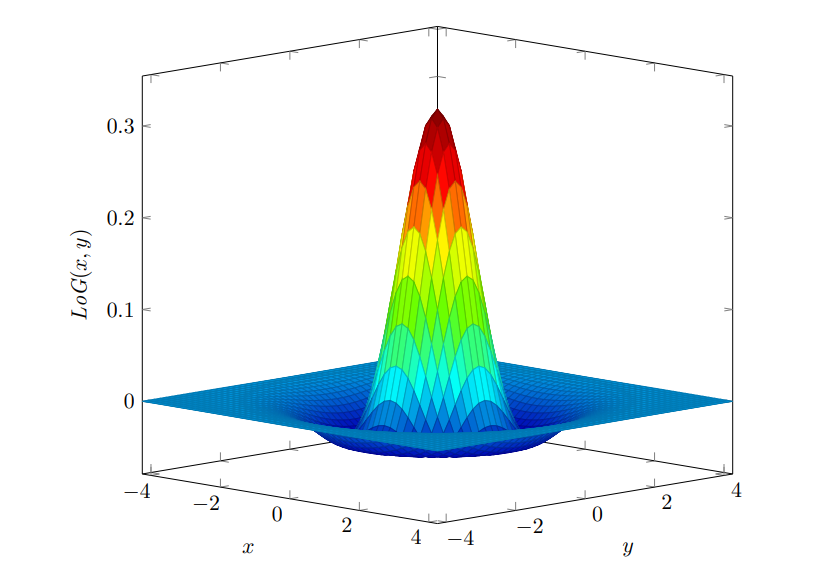
\includegraphics[]{images/LoG.png}
\end{center}
This new operator can be used in order to detect circular regions at different scales (blob detection). Basically, it highlights parts of the image with high contrast around a circular region.
\begin{center}
    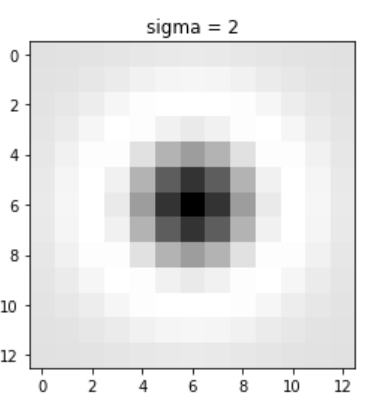
\includegraphics[scale = 0.8]{images/circular region loG.png}
\end{center}
As in the case of the Gaussian filter, we can fine-tune the $\sigma$ parameter in order to make the size of the circular region either bigger or smaller.
\begin{itemize}
    \item Increasing $\sigma$: More blur effect and larger size of the circular region.
    \item Decreasing $\sigma$: Less blur effect and smaller size of the circular region.
\end{itemize}
As usual, the corresponding kernel is a discrete approximation of the continuous function. \newline\newline
So, this filter can be used as the scale invariant function mentioned before, because it gives an high response if the circular region fits well the underlying image region\footnote{giving a high response means that the pixel values in the resulting image after the application of the filter are high.}. In order to find the circular region size that best fits a local feature at a given scale, we can apply this filter for different values of $\sigma$ (ideally all) and look for the one in which the filter gives the highest response.
\begin{center}
    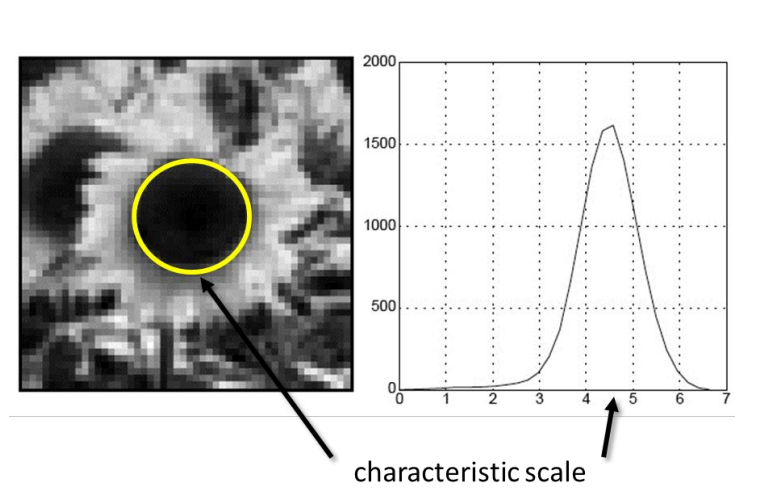
\includegraphics[scale = 0.8]{images/LoG scales.png}
\end{center}
Note that the filter is scale invariant but also rotation invariant, because it considers circular regions.

\subsection{Harris-Laplacian: Scale invariant detection}
Harris-Laplacian is a corner detection algorithm that applies Harris algorithm \textit{in space} (image coordinates) and the Laplacian of Gaussian over the different scales (changing the parameter $\sigma$). It can be used in order to detect local features across scales. \newline\newline
Let's say there is a $3 \times 3$ window. It computes Harris corner detection across different scales (images convolved with $LoG$ filters with different values of $\sigma$) and it detects as a key-point a pixel in which its value is the local maxima in its respective scale \textbf{and} also in the previous scale and in the next one. Basically, a key-point is compared with its respective 8 pixels neighborhood and with the 18 pixels from adjacent scales (9 pixels from each scale).
\begin{center}
    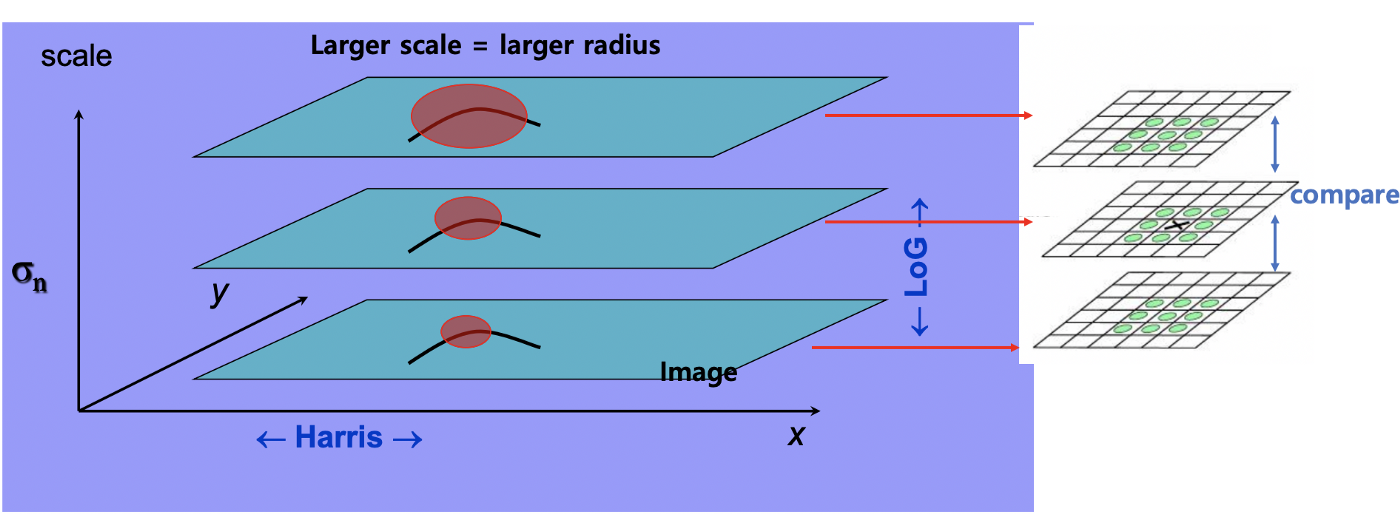
\includegraphics[scale = 0.3]{images/Harris-LoG.png}
\end{center}
This technique makes the Harris detector more robust to the scale changes.


\chapter{Local invariant features II}
\section{Difference of Gaussians (DoG)}
It is possible to define an approximation of the Laplacian of Gaussian by using difference of Gaussians:
\[DoG = G(x,y,k\sigma) - G(x,y,\sigma)\]
where $k$ is a scalar value and $G$ is the two-dimensional Gaussian function
\[\frac{1}{2\pi \sigma^{2}}e^{-\frac{x^{2} + y^{2}}{2\sigma^{2}}}\]
Basically, it approximates the behavior of the Laplacian of Gaussian computing the difference between two Gaussian functions with different values of $\sigma$
\begin{center}
    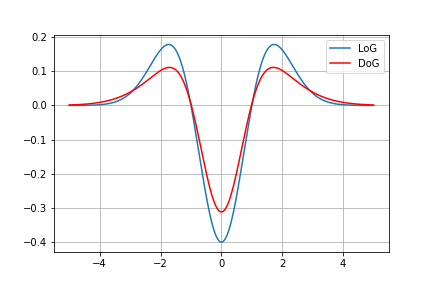
\includegraphics[scale = 0.7]{images/DoG Approx.png}
\end{center}
This is useful because $DoG$ is more efficient from a computational point of view. In fact, computing the second order derivative is more expensive than performing a difference between two functions.
\section{SIFT algorithm}
SIFT is a scale invariant feature detection algorithm that applies $DoG$ both in space and over different scales. Thanks to this, it is computationally more efficient than the Harris-Laplacian algorithm. Following are the major stages of computation used to generate the set of image features:
\begin{enumerate}
    \item \textbf{Scale-space extrema detection:} The first stage of computation searches for local features over all scales and image locations using a difference of Gaussian function.
    \item \textbf{Key-point localization:} At each candidate location, a detailed model is fit to determine location and scale. Key-points are selected based on measures of their stability (\textbf{It was not covered in class}).
    \item \textbf{Orientation assignment:} One or more orientations are assigned to each key-point location based on local image gradient directions.
    \item \textbf{Key-point descriptor:} Describing the key-points as a high dimensional vector such that it is highly distinctive and invariant as possible to variations such as changes in viewpoint, illumination, translation, rotation and scale.
\end{enumerate}
\begin{center}
    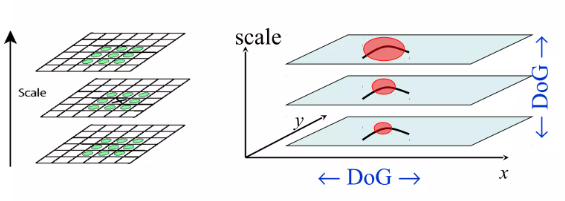
\includegraphics[]{images/DoG space scales.png}
\end{center}
\subsection{Scale-space peak Selection}
The initial image is repeatedly convolved with Gaussians with different values of $\sigma$ to produce a set of scale-space images. Adjacent Gaussian images are subtracted to produce the difference of Gaussian images. These $DoG$ images contain the details of the original image at different scales\footnote{look at the Sharpening filter and derivative of Gaussian sections}. This procedure creates the first \textbf{ octave of scale-space}. In order to find a good approximation of the Laplacian of Gaussian, this process is repeated multiple times and after each octave the Gaussian image is down-sampled by a factor of 2 (each octave’s image size is half the previous one).
\begin{center}
    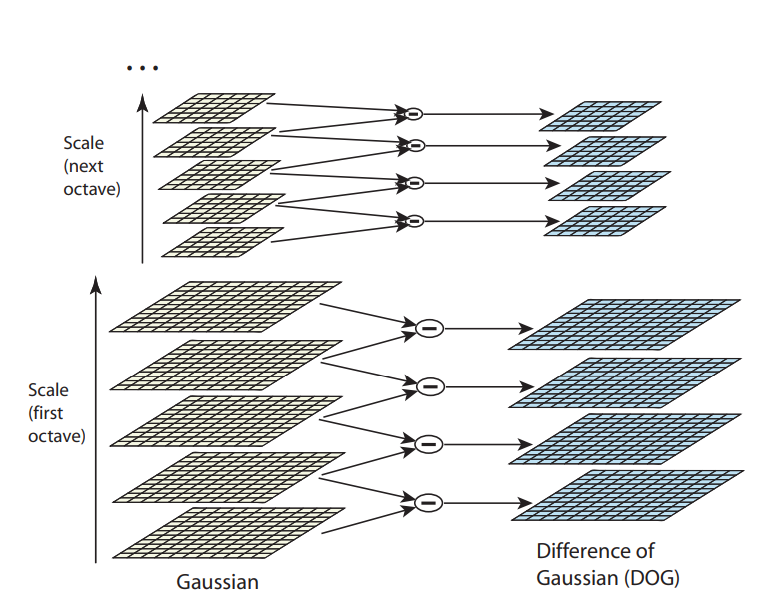
\includegraphics[scale = 0.9]{images/SIFT octaves.png}
\end{center}
Maxima and minima of the $DoG$ images are detected by comparing a pixel to its 26 neighbors in 3x3 regions at the current and adjacent scales (previous and next scales with respect to the current). A key-point is selected only if it is larger, in term of intensity, than all of these neighbors or smaller than all of them.
\begin{center}
    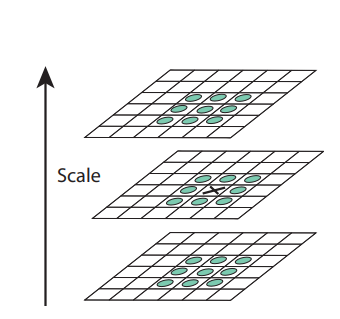
\includegraphics[]{images/SIFT DoG space.png}
\end{center}
Thanks to this, the local features detected are more robust also to some transformations across scales.
\subsection{Orientation assignment}
\label{subsection:orientation}
After the detection process we already know the scale at which each key-point was detected (parameter $\sigma$), so we have scale \textit{invariance}. By assigning a consistent orientation to each key-point based on local image properties, the
key-point descriptor can be represented relative to this orientation and therefore achieve invariance to image rotation.\newline\newline
An orientation histogram is formed from the gradient orientations of sample points within a region around the key-point (using the scale of the key-point to select the level of Gaussian blur for the image). The orientation histogram covers the 360 degree range of orientations. Each sample point added to the histogram is weighted by its gradient magnitude and by a Gaussian-weighted circular window. The highest peak in the histogram is selected as the dominant direction of the key-point and then any other local peak that is within 80\% of the highest peak is used to also create a key-point with that orientation. Therefore, for locations with multiple peaks of similar magnitude, there will be multiple key-points created at the same location and scale but different orientations.
\subsection{Key-point descriptor}
At this point, each key-point has a location, scale and orientation. The next step is to compute a descriptor for the local image region. To do this, a $16 \times 16$ window around the key-point is taken and it is divided into 16 sub-blocks of $4 \times 4$ size \footnote{The size of the window can be modified, $16 \times 16$ is the standard SIFT }. For each sub-block, an 8 bin orientation histogram is created following the procedure mentioned before (\ref{subsection:orientation}). Therefore, a descriptor will be a $4 \times 4 \times 8 = 128$ element feature vector.
\begin{center}
    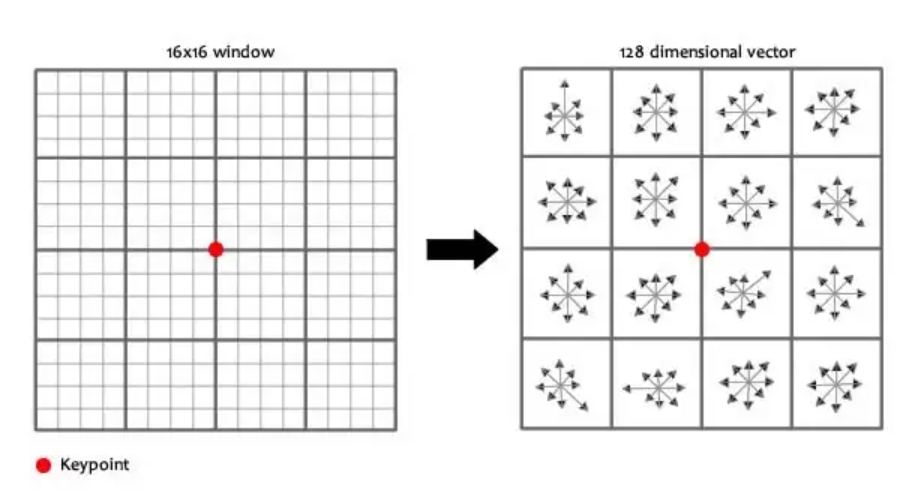
\includegraphics[scale = 0.7]{images/sift descriptor.png}
\end{center}
The feature vector uses gradient orientations, but if you rotate the image, these orientations change. So, in order to achieve orientation
invariance, the coordinates of the descriptor and the gradient orientations are rotated relative to the key-point orientation.
\subsection{Key-points matching}
A comparative evaluation of different scale invariant key-points detectors can be done by using the repeatability rate. It is defined as the ratio between the number of point-to-point correspondences that can be established for detected points and the number of all possible correspondences.
\begin{center}
    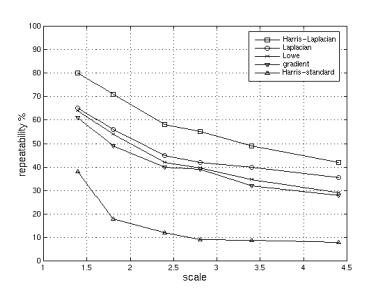
\includegraphics[scale = 1.3]{images/repeatability rate.png}
\end{center}
But how can we match key-points? One way to do it is by computing, for each descriptor in the first image, the Euclidean distance between this descriptor and all the descriptors of the second image and select the one with minimum distance. A more robust method can be, instead of looking only for the minimum distance, compute the ratio between the first two closest distances. If it is greater that 0.8, the match is rejected. 
\begin{center}
    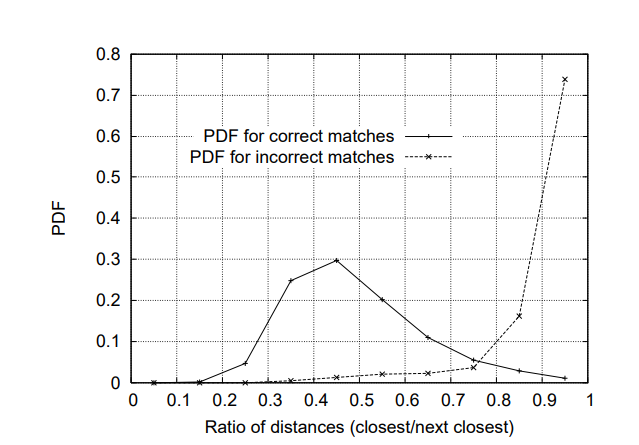
\includegraphics[]{images/ratio closest distances.png}
\end{center}
Now we can describe a pipeline to perform features matching:
\begin{enumerate}
    \item Detect key-points
    \item Build key-points descriptors
    \item Match key-point features
    \item Align images
\end{enumerate}


\chapter{Bag of Visual Words}
\section{Image classification pipeline}
In order to implement image classification, we need two major components:
\begin{itemize}
    \item A way to describe images. Not just local features descriptors, but a \textbf{global} representation of the image.
    \item A procedure to \textbf{compare} different images and learn a statistical model of a specific class. 
\end{itemize}

\subsection{Nearest Neighbor classifier}
The simplest way to \textit{learn} a model of a specific class is by using nearest neighbor technique.\newline\newline
Let's assume that we have just two classes (binary classification problem) and that we represented our training images into a feature space. The idea is to classify a new test image with the label of the closest training image (e.g. in terms of Euclidean distance) in the feature space.\newline\newline
This method has some problems:
\begin{itemize}
    \item If the test image is equally distant from two (or more) neighbors, a discriminant is needed for classification.
    \item It is very sensitive to outliers.
\end{itemize}
\subsection{k-Nearest Neighbors classifier}
A better generalization of the previous technique is the k-Nearest Neighbors classifier.\newline\newline
The image is assigned to the most common class among its k nearest neighbors (k is a positive integer, typically small). if k = 1, the method is equal to the Nearest Neighbor classifier.\newline\newline
This method solves the problems described before but it still has weakness. If k is too large and the dataset is too small, the model will be highly biased by the most frequent class. So, in order to work well, k-NN needs large datasets.
\section{Simple image representation}
The simplest representation is provided by raw pixels. We need to map all the images, despite the resolution, to the same dimensional feature space. Then we can represent images as a 2D or 1D array of pixels, define a distance (e.g. L1 or L2) to compare images and use k-NN for classification.\newline\newline
The L1 distance metric is defined as follows:
\[d_{L1}(I_{1}, I_{2}) = \sum_{p}|I_{1}^{p} - I_{2}^{p}|\]
\[ \begin{bmatrix}
    56 & 32 & 10 & 18\\
    90 & 23 & 128 & 133\\
    24 & 26 & 178 & 200\\
    2 &  0  & 255 & 220\\
\end{bmatrix}
-
\begin{bmatrix}
    10 & 20 & 24 & 17\\
    8  & 10 & 89 & 100\\
    12 & 16 & 178& 170\\
    4  & 32 & 233& 112\\
\end{bmatrix}
=
\begin{bmatrix}
    46 & 12 & 14 & 1\\
    82 & 13 & 39 & 33\\
    12 & 10 & 0 & 30\\
    2 & 32 & 22 & 108\\
\end{bmatrix}
\rightarrow
456
\]
Following this pipeline, we obtain a model that is fast for training (it just only needs to memorize training data for k-NN) but slow for predictions, because it needs to compute the distance, for each test image, between the current image and all the training images. This is bad because the goal is to find a model that has slow training time and fast prediction time.\newline\newline
A better result can be achieved by doing the following things:
\begin{itemize}
    \item Use a better image representation
    \item Rely on better functions to compare images
    \item Use better classifiers
\end{itemize}
\section{Bag of Visual Words}
Bag Of Visual Words is a technique to describe images. The approach has its origin in text retrieval and it is an extension of the Bag of Words algorithm. In Bag Of Words, we scan through the entire document and keep a count of each word appearing in the document. Then, we create a histogram of frequencies of words and use it to describe the text document. In Bag Of Visual Words, our input are images and we use \textbf{visual words} to describe them.
\newline\newline
The pipeline follows these steps:
\begin{enumerate}
    \item Extract local features (e.g. using SIFT) from training images.
    \item Quantize the feature space (build a visual dictionary or codebook). Make this operation via clustering algorithms such as K-means. The center points, that we get from the clustering algorithm, are our visual words.
    \item For each feature of each training image, find the closest visual word in the visual dictionary and build frequency histograms (one for each training image).
    \item Compute histograms of visual words of \textbf{test} images (following the same procedure) and predict their class using the histograms of training images (e.g. using k-NN).
\end{enumerate}
\subsection{Feature extraction}
Note that features extracted using SIFT will be mostly around the object, so, in some cases it could be a better idea to use a feature extraction algorithm that takes into account also the background (e.g. even random sampling).
\subsection{Visual dictionary}
After the feature extraction step, we have a list of feature descriptors (e.g. SIFT descriptors) that contains the descriptors of all the images. These descriptors are used as input of a clustering algorithm such as k-means. This algorithm forms k clusters and returns the center of each group. Each cluster center is a visual word and all these k visual words form the visual dictionary.\newline\newline
\textbf{k-means clustering:} The goal is to minimize sum of square Euclidean distances between points $x_{i}$ and their nearest cluster centers $m_{k}$
\[D(x,m) = \sum_{k}\sum_{i \in k}(x_{i} - m_{k})^{2}\]
Application of Lloyd's algorithm:
\begin{enumerate}
    \item Randomly initialize $\textbf{K}$ cluster centers
    \item Iterate until convergence
    \begin{enumerate}
        \item Assign each data point to the nearest center
        \item Recompute each cluster center as the mean of all points assigned to it
    \end{enumerate}
\end{enumerate}
How to choose the parameter $K$ of the algorithm?
\begin{itemize}
    \item Too small: visual words not representative of all patches.
    \item Too large: quantization artifacts, overfitting.
\end{itemize}
\subsection{Create histograms}
At this point, we create histogram of visual words of each image. This assignment step can be done in two ways:
\begin{itemize}
    \item \textbf{Hard assignment:} For each feature in the image, find the closest visual word in the visual dictionary and increase by one the count of that particular word.
    \item \textbf{Soft assignment:} Weigh frequent and infrequent words differently. A visual word that appears often is less useful for matching, so it will have a small weight attached to it. On the other hand, an infrequent word will have a bigger weight.\newline\newline
    This concept is inherited from Bag of Words for text retrieval. Instead of computing regular histogram distance, we weight each word by its inverse Document Frequency such as:
    \begin{center}
        IDF of word $j$: log ( \textit{number of documents / number of documents in which $j$ appears)}
    \end{center}    
\end{itemize}
\subsection{Classification}
After creating histograms of visual words both for testing and training images, use any classification model (k-NN, SVM, ...) to perform classification. 

\subsection{Spatial information}
In Bag of Visual Words spatial information is lost. In order to reintroduce it, we can use spatial pyramids. Instead of having one-level histogram, we iterate the procedure at different levels of spatial resolution.
\begin{itemize}
    \item Pyramid is built by using multiple copies of the image.
    \item Each level is 1/4 of the size of the previous level.
    \item The lowest level is the one with the highest resolution.
    \item The highest level is the one with the lowest resolution.
\end{itemize}
\begin{center}
    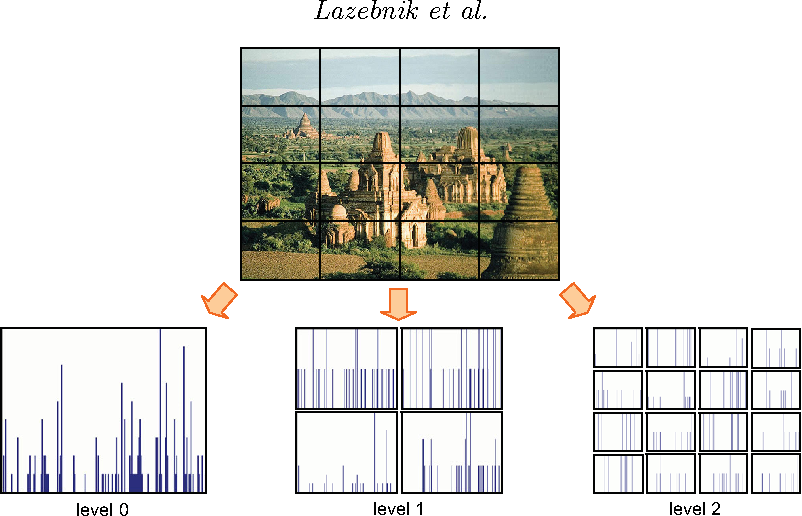
\includegraphics[scale = 0.4]{images/Spatial pyramids.png}
\end{center}


\chapter{CNN I}
\section{Neural Networks}
An Artificial Neural Network is a system consisting of interconnected units that compute nonlinear functions.
\begin{itemize}
    \item \textbf{input} units represent input variables.
    \item \textbf{output} units represent output variables.
    \item \textbf{hidden} units represent internal variables that codify (after learning) correlations among input and desired output variables.
    \item \textbf{weights} are associated to connections between units.
\end{itemize}
Multiple layers of cascaded units makes a Neural Network able to implement complex non linear functions. The non linearity of the model is given by the activation functions. In fact, without them (linear activation) the result of the model, even if it’s very complex, would still be linear.
\begin{itemize}
    \item \textbf{Sigmoid:}
    \[\frac{1}{1 + e^{-y}}\]

    \item \textbf{ReLU:}
    \[max(0, y)\]
    
    \item \textbf{tanh:}
    \[tanh(x)\]

    \item \textbf{Leaky ReLU:}
    \[max(0.1x, x)\]
\end{itemize}
The basic idea of the learning algorithm consists in two phases:
\begin{itemize}
    \item \textbf{Forward phase:} for each example in the training set, present it to the network and compute the output. Each neuron performs a dot-product with the input and its weights, adds the bias and applies the \textbf{activation function}.
    
    \item \textbf{Backward phase:} Back-propagate the committed error and update the weights of the hidden units accordingly. 
\end{itemize}
\textbf{Back-propagation} is an algorithm based on the gradient descent method that aims to update the weights of a Neural Network in order to minimize the error between the predicted output and the true output. The algorithm works by propagating the error back through the network, starting with the output layer and moving backwards through the hidden layers, adjusting the weights at each layer to reduce the error. It can be implemented in different ways:
\begin{itemize}
    \item \textbf{Batch gradient descent:} It \textbf{cumulates} gradients over all the training examples and then updates the weights.
    \item \textbf{Stochastic gradient descent:} For each example in $S$, it computes the gradients and update the weights.
    \item \textbf{Mini-batch gradient descent:} It updates the weights considering a subset of examples $Q \subseteq S$. 
\end{itemize}
This process is typically repeated many times until the error is sufficiently small or the maximum number of iterations is reached. Let's define the algorithm according to the derivations seen before:

\section{Convolutional Networks}
Convolutional networks, also known as convolutional neural networks or CNNs, are a specialized kind of neural network for processing data that has a known, grid-like topology. Examples include time-series data, which can be thought of as a 1D grid taking samples at regular time intervals, and image data, which can be thought of as a 2D grid of pixels. Convolutional networks have been tremendously successful in practical applications. The name “convolutional neural network” indicates that the network employs a mathematical operation called convolution. The idea is to substitute matrix multiplication with convolution.\newline\newline
Images have three properties that suggest the need for specialized architecture:
\begin{itemize}
    \item they are high-dimensional, e.g. 224×224 RGB values (i.e., 150,528 input dimensions). Hidden layers in fully connected networks are generally larger than the input size, and so even for a shallow network, the number of weights would exceed 150,528! or 22 billion. Obvious practical problems in terms of the required training data, memory, and computation.

    \item Nearby image pixels are statistically related. Fully connected networks have no notion of “nearby” and treats the relationship between every input equally; if the pixels of the training and test images were randomly permuted in the same way, the network could still be trained with no practical difference.

    \item The interpretation of an image is stable under geometric transformations. An image of a tree is still an image of a tree if we shift it leftwards by a few pixels. However, this shift changes every input to the network, and so the model would have to learn the patterns of pixels that correspond to a tree separately at every position. This is clearly inefficient.
\end{itemize}
Convolutional networks are perhaps the greatest success story of biologically
inspired artificial intelligence. Neurophysiologists
David Hubel and Torsten Wiesel collaborated for several years to determine many of the most basic facts about how the mammalian vision system works. They observed how neurons in the cat’s brain responded to images projected
in precise locations on a screen in front of the cat. Their great discovery was that neurons in the early visual system responded most strongly to very specific patterns of light, such as precisely oriented bars, but responded hardly at all to other patterns.

\subsection{Convolution operator}
In its most general form, \textbf{convolution} is an operation on two functions of a real-valued argument. To motivate the definition of convolution, we start with examples of two functions we might use.\newline\newline
Suppose we are tracking the location of a spaceship with a laser sensor. Our
laser sensor provides a single output $x(t)$, the position of the spaceship at time $t$. Both $x$ and $t$ are real-valued, i.e., we can get a different reading from the laser sensor at any instant in time.\newline\newline
Now suppose that our laser sensor is somewhat noisy. To obtain a less noisy
estimate of the spaceship’s position, we would like to average together several measurements. Of course, more recent measurements are more relevant, so we will want this to be a weighted average that gives more weight to recent measurements. We can do this with a weighting function $w(a)$, where $a$ is the age of a measurement. If we apply such a weighted average operation at every moment, we obtain a new function $s$ providing a smoothed estimate of the position of the spaceship:

\[s(t) = \int_{-\infty}^{\infty} x(a)w(t - a)da\]
The convolution operation is typically denoted with an asterisk:
\[s(t) = (x \,*\, w)(t)\]
In convolutional network terminology, the first argument (in this example, the function $x$) to the convolution is often referred to as the \textbf{input} and the second argument (in this example, the function $w$) as the \textbf{kernel} (needs to be a valid probability density function). The output is sometimes referred to as the \textbf{feature map}.\newline\newline
Usually, when we work with data on a computer, time will be discretized:
\[s(t) = (x \,*\, w)(t) = \sum_{a = - \infty}^{\infty}x(a)w(t-a)\]
In machine learning applications, the input is usually a multidimensional array of data and the kernel is usually a multidimensional array of parameters that are adapted by the learning algorithm.\newline\newline
We often use convolutions over more than one axis at a time. For
example, if we use a two-dimensional image $I$ as our input, we probably also want to use a two-dimensional kernel $K$:
\[S(i, j) = (I \, *\, K)(i, j) = \sum_{a = -m}^{m}\sum_{b = -n}^{n}K(a, b)I(i - a, j - b)\]
\begin{center}
    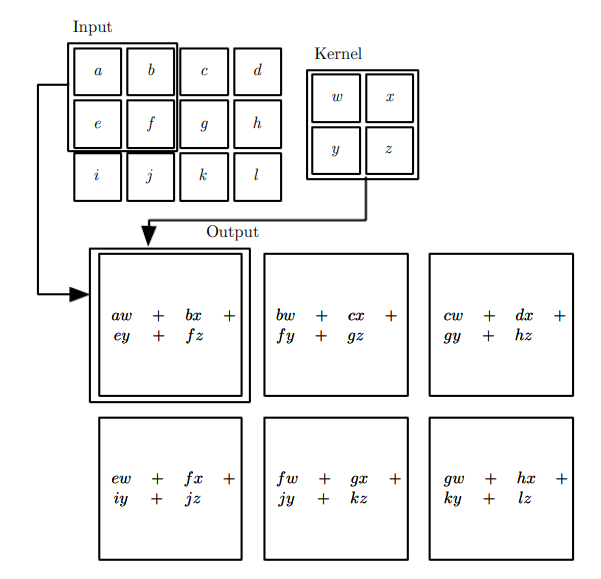
\includegraphics[scale=0.7]{images/Cross-corr.png}
\end{center}
From the example above we can notice two things:
\begin{itemize}
    \item The kernel is applied as a sliding window across the image.

    \item Actually, the operator applied in the example is not convolution, but \textbf{cross-correlation:}
    \[S(i, j) = \sum_{a = -m}^{m}\sum_{b = -n}^{n}K(a, b)I(i + a, j + b)\]
    In fact, we apply convolution by \textbf{flipping} the kernel relative to the input, in the sense that as $b$ increases, the index into the input decreases, but the index into the kernel increases. Many machine learning libraries implement cross-correlation but call it convolution.
\end{itemize}
The main properties of convolution are:
\begin{itemize}
    \item Sparse interactions $\rightarrow$ kernel smaller than input, efficiency.

    \item Parameter sharing

    \item Equivariant representations

    \item Works with inputs of variable size
\end{itemize}

\subsection{Sparse interactions}
Traditional neural network layers use matrix multiplication, having a matrix of parameters with a separate parameter describing the interaction between each input unit and each output unit. Convolutional networks, however, typically have sparse interactions (also referred to as sparse connectivity or sparse weights). This is accomplished by making the kernel smaller than the input. This means that we need to store fewer parameters, which both reduces the
memory requirements of the model and improves its statistical efficiency. It also means that computing the output requires fewer operations.
\begin{center}
    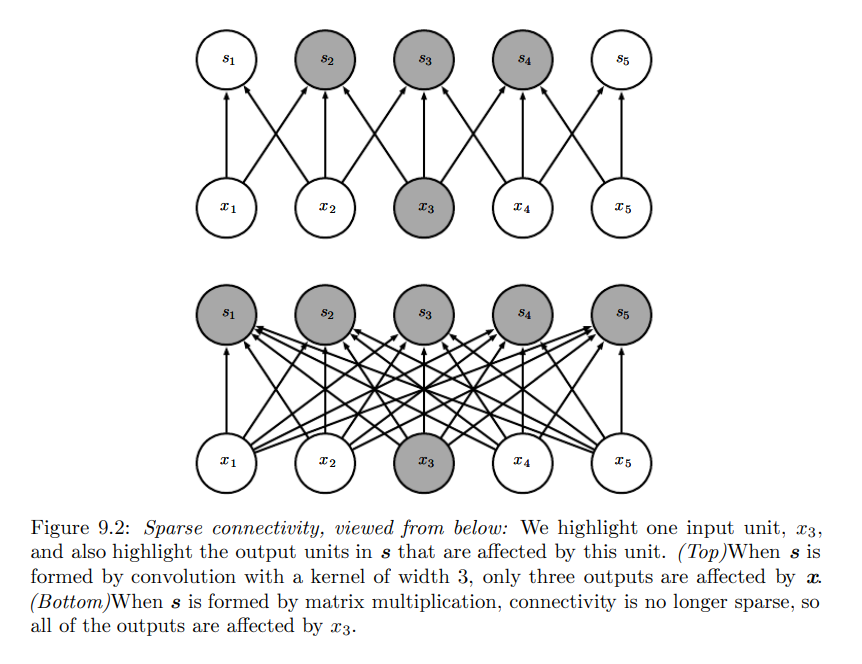
\includegraphics[scale = 0.7]{images/Sparse-conn.png}
\end{center}
The receptive field of the units in the deeper layers of a convolutional network is larger than the receptive field of the units in the shallow layers. This means that even though direct connections in a convolutional net are very sparse, units in the deeper layers can be indirectly connected to all or most of the input. This allows the network to efficiently describe complicated interactions between many variables by constructing such interactions from simple building blocks that each describe only sparse interactions.
\begin{center}
    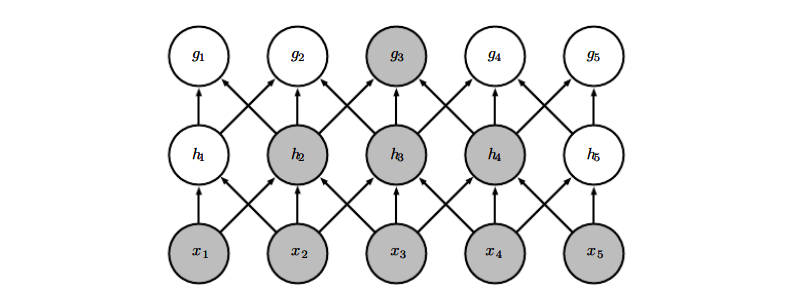
\includegraphics[scale=0.7]{images/receptive field.png}
\end{center}

\subsection{Parameter sharing}
\textbf{Parameter sharing} refers to using the same parameter for more than one function in a model. In a traditional neural net, each element of the weights' matrix is used exactly once when computing the output of a layer. In a convolutional neural net, each member of the kernel is used at every position of the input (except perhaps some of the boundary pixels, depending on the design decisions regarding the boundary). The parameter sharing used by the convolution operation means that rather than learning a separate set of parameters for every location, we learn only one set. It further reduces the storage requirements of the model to $k$ parameters (just the filter), with $k$ several order of magnitude smaller than the input size. Convolution is thus dramatically more efficient than dense matrix multiplication in terms of the memory requirements and statistical efficiency.
\begin{center}
    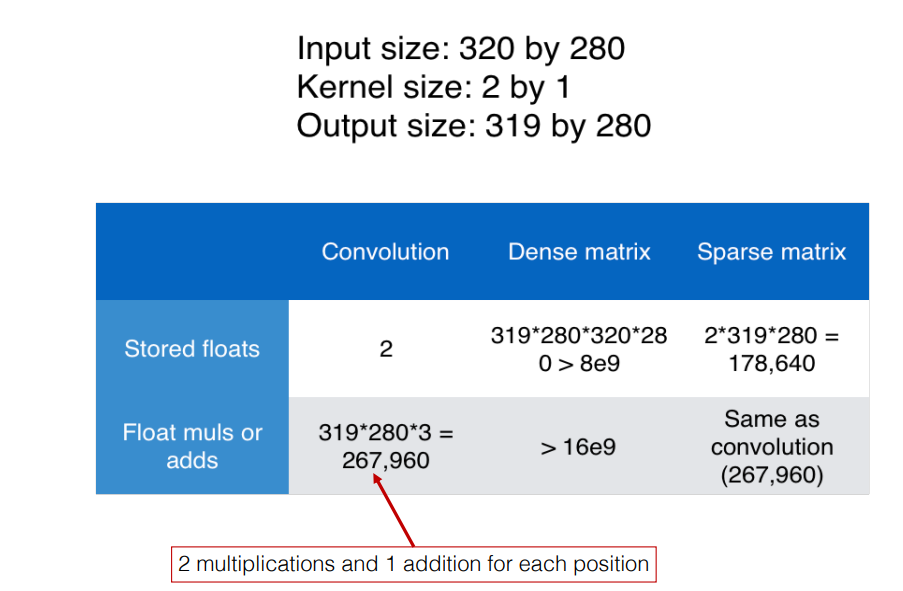
\includegraphics[scale=0.7]{images/conv-efficiency.png}
\end{center}

\subsection{Equivariance to translation}
In the case of convolution, the particular form of parameter sharing causes the layer to have a property called \textbf{equivariance} to translation. To say a function is
equivariant means that if the input changes, the output changes in the same way. Specifically, a function $f(x)$ is equivariant to a function $g$ if $f(g(x)) = g(f(x))$. In the case of convolution, if we let $g$ be any function that translates the input, i.e., shifts it, then the convolution function is equivariant to $g$. For example, with images, convolution creates a 2-D map of where certain features appear in the input. If we move the object in the input, its representation will move the
same amount in the output. Basically, due to parameter sharing, the kernel detects a feature regardless of where the feature is in the input image.\newline\newline
Convolution is not naturally equivariant to some other transformations, such as changes in the scale or rotation of an image. Other mechanisms are necessary for handling these kinds of transformations.

\subsection{Inputs of variable size}
Consider a collection of images, where each image has a different
width and height. It is unclear how to model such inputs with a weight matrix of fixed size. Convolution is straightforward to apply; the kernel is simply applied a different number of times depending on the size of the input, and the output of the convolution operation scales accordingly.

\subsection{Strided Convolution}
We may want to skip over some positions of the kernel in order to reduce the
computational cost (at the expense of not extracting our features as finely).
We can think of this as downsampling the output of the full convolution function. We can do this by sampling only every $s$ pixels in each direction in the output. We refer to $s$ as the \textbf{stride} of this downsampled convolution. It is also possible to define a separate stride for each direction of motion.
\begin{center}
    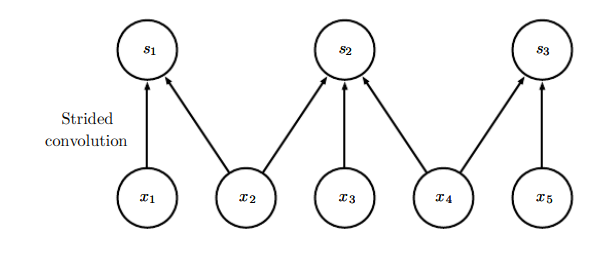
\includegraphics[scale=0.7]{images/stride.png}
\end{center}

\subsection{Dilated Convolution}
Increasing the kernel size has the disadvantage of requiring more weights. In order to reduce the number of stored weights we can use \textbf{dilated convolution}, that is, the kernel values are spaced with zeros. In 1D we can turn a kernel of size five into a dilated kernel of size three by setting the second and fourth elements to zero. We still integrate information from a larger input region but only require three weights to do this. The number of zeros we intersperse between the weights is termed the dilation rate.

\subsection{Pooling}
A typical layer of a convolutional network consists of three stages. In the first stage, the layer performs several convolutions in parallel to produce a set of linear activations. In the second stage, each linear activation is run through a nonlinear activation function, such as the rectified linear activation function. In the third stage, we use a pooling function to modify the output of the layer further.\newline\newline
A pooling function replaces the output of the net at a certain location with a summary statistic of the nearby outputs. For example, the \textbf{max pooling} operation reports the maximum output within a rectangular neighborhood. Another popular pooling function is the average of a rectangular neighborhood.
\begin{center}
    \includegraphics[]{images/cnn-structure.png}
\end{center}
In all cases, pooling helps to make the representation become approximately invariant to small translations of the input. Invariance to translation means that if we translate the input by a small amount, the values of most of the pooled outputs do not change. Furthermore, pooling reduces the size of the input of the subsequent layers, thus it improves efficiency.\newline\newline
For many tasks, pooling is essential for handling inputs of varying size.

\subsection{Padding}
Given an $n \times n$ kernel, its external row/column coincides with the border of the image when the center of this mask is at distance $\frac{n-1}{2}$ from the edge. If you move further out, part of the window \textit{leaves} the image.\newline
This situation can be managed in three different ways:
\begin{itemize}
    \item limit the movement of the mask, keeping it at a minimum distance of $\frac{n-1}{2}$ from the edges.
    \item duplicate the external rows/columns of the image
    \item enlarge the image with rows/columns of zeros
\end{itemize}
Solution 1 gives reliable results, but produces a different size image from the original. Solutions 2 and 3, on the other hand, give results that are not exactly authentic near the edges, but are often convenient because they allow you to obtain an output image with the same size as the input one.

\subsection{Multi-channel input}
\begin{center}
    \includegraphics[]{images/multi-channel input.png}
\end{center}


\subsection{Unshared convolution}
In some cases, we do not actually want to use convolution, but rather locally connected layers. This is sometimes also called \textbf{unshared convolution}, because it is a similar oper- ation to discrete convolution with a small kernel, but without sharing parameters across locations. Locally connected layers are useful when we know that each feature should be
a function of a small part of space, but there is no reason to think that the same feature should occur across all of space.

\subsection{Structured Outputs}
Convolutional networks can be used to output a high-dimensional, structured
object, rather than just predicting a class label for a classification task or a real value for a regression task. Typically, this object is a tensor with the same shape of the input, with a class label for each pixel to produce object detection masks.


\end{document}
